\documentclass[10pt]{sig-alternate-05-2015}
%\documentclass{sig-alternate-05-2015}
%\documentclass{sig-alternate-10pt}
\usepackage[breaklinks=true,colorlinks=true,plainpages=false,citecolor=blue,urlcolor=blue,linkcolor=magenta,filecolor=blue]{hyperref}
\usepackage{url}        % Not compatible with hyperref?
\usepackage{float}
\usepackage{graphicx}
\usepackage{amsmath}
\usepackage{color}
\usepackage{times}
\usepackage[sort]{natbib}
\usepackage{enumitem}
%\usepackage{subfigure}
\usepackage{verbatim}
\usepackage{xspace}
\usepackage{xfrac}
\usepackage{algorithmic} % must come after hyperref
\usepackage{algorithm}
%ejr ac/dc 
\usepackage{marvosym}
\let\marvosymLightning\Lightning

\usepackage{lastpage}

\usepackage[utf8]{inputenc}
\usepackage{cleveref}
\crefname{section}{§}{§§}
\Crefname{section}{§}{§§}
\crefformat{section}{§#2#1#3}

\usepackage{listings}
%\usepackage{microtype} %does typographical voodoo to get rid of most overfull
                       %boxes. Ideally requires pdfTeX 1.4+, going directly
                       %to pdf. Don't use a DVI workflow.
\usepackage{balance}   %\balance keywork has to be included in the last page that
                       % will not be balanced, in the first column.
\usepackage{datetime}
\usepackage{morefloats}

\usepackage{caption}
\usepackage{subcaption}
\usepackage{multirow}

\DeclareMathVersion{mathchartertext}
\SetSymbolFont{letters}{normal}{OML}{mdbch}{m}{n}
\newcommand{\gchar}[1]{\mathversion{mathchartertext}$#1$\mathversion{normal}}

% Configure algorithmic and listings
\renewcommand{\algorithmicrequire}{\textit{Input:}}
\renewcommand{\algorithmicensure}{\textit{Output:}}
\lstset{%language=Python,
numberstyle=\footnotesize,
basicstyle=\ttfamily\scriptsize,
numbers=left,
stepnumber=1,
showstringspaces=false,
breaklines=true}

 \newcommand{\todo}[1]{\textcolor{blue}{\textbf{TODO:} #1}}
 \newcommand{\eric}[1]{\textcolor{red}{\textbf{Eric:} #1}}
 \newcommand{\aditya}[1]{\textcolor{red}{\textbf{Aditya:} #1}}
 \newcommand{\keqiang}[1]{\textcolor{red}{\textbf{Keqiang:} #1}}
\newcommand{\cut}[1]{}


%camera ready submission (crs)
%\newcommand{\crs}[1]{\textcolor{blue}{#1}} %show changes
\newcommand{\crs}[1]{#1}% Do nothing

%\newcommand{\todo}[1]{}
\newcommand{\jeff}[1]{}
\newcommand{\colin}[1]{}
\newcommand{\brent}[1]{}

%\newcommand{\eg}{\emph{e.g.}\xspace}
\newcommand{\eg}{{e.g.}\xspace}
\newcommand{\cf}{{cf.}\xspace}
%\newcommand{\ie}{\emph{i.e.}\xspace}
\newcommand{\ie}{{i.e.}\xspace}
\newcommand{\etal}{{et al.}\xspace}
%\newcommand{\acdc}{{LiquidSwitch}\xspace}
\newcommand{\acdc}{{AC\text{\marvosymLightning}DC}\xspace}
%\newcommand{\acdc}{{AC/DC}\xspace}
\newcommand{\cwnd}{{{\tt CWND}}\xspace}
\newcommand{\rwnd}{{{\tt RWND}}\xspace}

\hyphenation{light-weight}
\hyphenation{meas-ure-ment}
\newcommand{\tightparagraph}[1]{\vspace{5pt}\noindent\textbf{#1}\ }

%ejr, adding per jitu's email
\setlength{\pdfpagewidth}{8.5in}
\setlength{\pdfpageheight}{11in}




%\title{Presto: Distributed Flowcell Load Balancing at the \\ Datacenter Network Edge}

%\title{AC{\LARGE \marvosymLightning{}}DC TCP: Virtual Switch-based Congestion Control Enforcement for Datacenter Networks}
\title{AC/DC TCP: Virtual Congestion Control Enforcement for Datacenter Networks}
%\author{Paper \#267,~\pageref{LastPage} pages}

\author{
{Keqiang He$^\dagger$ \hspace{0.2in} Eric Rozner$^\ddag$ \hspace {0.2in} Kanak Agarwal$^\ast$ \hspace {0.2in} Yu (Jason) Gu$^\ast$}\\[.2cm]
{Wes Felter$^\ddag$ \hspace{0.1in} John Carter$^\ast$ \hspace{0.1in} Aditya Akella$^\dagger$}\\\\
{\affaddr{$^\dagger$University of Wisconsin--Madison \hspace{0.15in} $^\ddag$IBM Research \hspace{0.15in} $^\ast$IBM }} %\\\\
%{\textcolor{red}{\normalsize Git-hash: \input{.git/ORIG_HEAD}}} \\
%{\textcolor{red}{\normalsize \today, \currenttime}}
}

%don't want date printed
\date{}

\newfont{\mycrnotice}{ptmr8t at 7pt}
\newfont{\myconfname}{ptmri8t at 7pt}
\let\crnotice\mycrnotice%
\let\confname\myconfname%


\clubpenalty=10000
\widowpenalty = 10000

\begin{document}

\CopyrightYear{2016}
\setcopyright{acmlicensed}
\conferenceinfo{SIGCOMM '16,}{August 22 - 26, 2016, Florianopolis , Brazil}
\isbn{978-1-4503-4193-6/16/08}\acmPrice{\$15.00}
\doi{http://dx.doi.org/10.1145/2934872.2934903}


\maketitle

\begin{abstract}

Multi-tenant datacenters are successful because tenants 
can seamlessly port their applications and services
to the cloud. Virtual Machine (VM) technology plays an integral role in this success
by enabling a diverse set of software to be run on a unified underlying framework. This
flexibility, however, comes at the cost of dealing with out-dated, inefficient, or 
misconfigured TCP stacks implemented in the VMs. This paper investigates if
administrators can take control of a VM's TCP congestion control
algorithm {\em without} making changes to the VM or network hardware.
We propose~\acdc{} TCP, a scheme that exerts fine-grained
control over arbitrary tenant TCP stacks by enforcing per-flow congestion
control in the virtual switch (vSwitch). Our scheme is light-weight, flexible, scalable and
can police non-conforming flows. In our evaluation the computational overhead
of~\acdc{} TCP is less than~\crs{one percentage point} and we show implementing an administrator-defined congestion control algorithm
in the vSwitch (\ie{}DCTCP) closely tracks its native performance, regardless of the VM's TCP stack. 


\end{abstract}


\begin{CCSXML}
<ccs2012>
<concept>
<concept_id>10003033.10003039.10003048</concept_id>
<concept_desc>Networks~Transport protocols</concept_desc>
<concept_significance>500</concept_significance>
</concept>
</ccs2012>
\end{CCSXML}

\ccsdesc[500]{Networks~Transport protocols}
\printccsdesc

\keywords{Datacenter Networks; Congestion Control; Virtualization;}
\chapter{Introduction}
\label{chap:intro}
Over the past few years, cloud-based networking solutions have been gaining widespread acceptance and
deployment for organizations such as enterprises and institutions~\cite{paxson1997end}.

\section{Cloud Infrastructure Organization}
% virtual network data plane

%While our work applies to general cloud networking settings, for the purposes of 
In this thesis, we focus on multi-tenant cloud data centers.
In this setting, tenants deploy \emph{virtual private clusters}
composed of application end-points (this could be service software in

\section{Challenges in Diagnosing Cloud Networks}
\label{sec:intro:challenges}
Troubleshooting network problems is difficult. A network is a distributed

\begin{itemize}
\item Cloud networks have higher complexity than traditional networks.  In data planes, network virtualization introduces more software components, including software switches, hypervisors, and so on; software middleboxes are introduced to support network function virtualization. In control planes, the cloud controllers need to perform more functions to set up virtual networks; the controllers map tenants' requirements from a logical view to a physical view, and finally to devices rules. Cloud networks involve a greater number of components involved, and these components may have logical or physical dependency (e.g., exchanging data or sharing hardware resources). This complexity in cloud networks makes them not only more error-prone but also difficulty to manage and diagnose.
\item The two roles in cloud networks makes the management trickier than traditional network. The two roles are the provider (or operator) and the tenants, and their information is isolated from each
other. In the case of network problems, the interaction between the provider and
the tenants is crucial for problem solving; however, this process is usually of low efficiency. 
The tenants observe misbehaviors of their applications directly, but they lack diagnostic tools.
The provider does not know the applications' performance, so they can only wait for tenants' tickets.
%Due to the isolation, both parties cannot perform a complete diagnosis; therefore, 
The two parties need to exchange observations to figure out the problem. This manual process increases
the problem-solving time and maintenance cost.
\item The visibility of cloud networks is not well provided to customers and operators. In traditional networks, network devices and components provide various information for operators to monitor or troubleshoot, e.g., packet drop statistics in switches and the network protocol stack. However, by our study, this kind of visibility is not well preserved in cloud networks. For customers, the cloud provider does not provide visibility of how their packets traverse the network for security reasons. For the provider, some virtualization components are introduced to cloud networks without keeping the visibility for diagnosis\textemdash there are several silent packet drops in VM hypervisors and software middleboxes. This is partially due to the fact that developers typically focus on functionality instead of diagnostic features in the first few versions of the software.
\end{itemize}


\section{An Overview of Our Approach}
\label{sec:intro:approach}
Ever since the birth of networks, network problems have been appearing and upseting network operators. There have been numerous proposals aiming to solve various problems. For example, there are standards or technologies such as SNMP, sFlow, and NetFlow to collect states in networks; there are network models and diagnostic algorithms to discover culprits in network problems; and there are various network diagnostic solutions for traditional networks and software-defined networks, which combine the technologies and algorithms. These approaches are undoubtedly valuable in their specific scenarios.

However, these solutions do not overcome the challenges in diagnosing cloud networks (Section~\ref{sec:intro:challenges}). In this thesis, we make a study of problems in cloud networks. According to the cloud organization, we look into each planes and summarize new problems. In more details, we found that in application planes, the isolation between tenants and the provider causes tenants unable to diagnose their virtual networks, thus we propose, design and implement a virtual network diagnostic service in application planes. We found that in data planes, increasing complexity and lack of visibility cause performance problems difficult to be identified, thus we modify software data planes, collect statistics and leverage the statistics to perform accurate diagnosis. We also find inconsistency issues in control planes, where tenant requirements may not be consistency with physical device states; we leave this problem in future works.

Decomposing cloud networks into three planes and reconsidering diagnostic challenges in cloud networks is an efficient way to discover, abstract and solve cloud network problems. We feel that, owing to our approach, several cloud-specific problems are discovered. Therefore, our works improve the reliability of cloud networks.

\section{Thesis Outline}
\label{sec:intro:outline}
The rest of this thesis is organized as follows. 
In Chapter~\ref{chap:background}, we make a study of cloud network problems and briefly describe our approaches.
In Chapter~\ref{chap:vnd},
we describe our design of the virtual network diagnostic service. In Chapter~\ref{chap:perfsight},
we present our solution for software data plane diagnosis.
In Chapter~\ref{chap:related}, we discuss the related work, 
Finally in Chapter~\ref{chap:conc}, we conclude this thesis and discuss options for future work.

\section{Design Decisions and Challenges}
\label{sec:background}

In Presto, we make several design choices to 
build a highly robust and scalable system that provides near optimal load 
balancing without requiring changes to the transport layer or switch hardware. We 
now discuss our design decisions.


\subsection{Design Decisions}

\tightparagraph{Load Balancing in the Soft Edge} A key design decision in Presto 
is to implement the functionality in the soft edge (\ie{}the vSwitch and hypervisor) of 
the network. 
%should we motivate why not to do it in hardware?
%A current trend in datacenter design is to utilize network equipment from 
%original design manufacturers (ODMs) in order to simplify and customize
%the network. This has been reported to significantly reduce costs and improve
%network performance~\cite{aws-peek}.
%Motivation here is that network is becoming very simple, and functionalities
%are being moved to an intelligent edge. Examples are VMWare/NSDI, Fabric, NFV in vSwitch,
%SDNs/OpenFlow, 
% Given recent advancements in this space\eric{what advancements? can we be more specific
% in order to provide better motivation?}, we believe the soft edge is the best 
% place to deploy new network functions, such as load balancing, in a scalable and 
% distributed manner.\eric{is this a new position? vmware nsdi paper...}
The vSwitch occupies a unique position in the networking stack 
in that it can easily modify packets without requiring any changes to customer VMs or transport layers.
Functionality built into the vSwitch can be made aware of the underlying hardware offload
features presented by the NIC and OS, meaning it can be fast.
Furthermore, an open, software-based approach prevents extra hardware cost and vendor 
lock-in, and allows for simplified network management. 
These criteria are important for providers today~\cite{aws-peek}.
Thanks to projects like Open vSwitch, 
soft-switching platforms are now fast, mature, open source, adopted widely, remotely 
configurable, SDN-enabled, and feature-rich~\cite{ovs-edge,nv-mtd,pfaff2015design}. Presto is built on these 
platforms.

\tightparagraph{Reactive vs Proactive Load Balancing} The second major design decision in 
Presto is to use a proactive approach to congestion management. Bursty 
behavior can create transient congestion that must be reacted to 
before switch buffers overflow to prevent loss (timescales range from 100s of $\mu$s 
to around 4 ms~\cite{planck}). This requirement renders most of the centralized reactive schemes ineffective
as they are often too slow to react to any but the largest network events,~\eg{}link failures. 
%Not reacting to transient congestion can increase tail latencies.
Furthermore, centralized schemes can hurt performance when rerouting
flows using stale information.
%By reacting on a different scale than the congestion, centralized schemes may reroute flows
%on stale information, which can hurt performance.
Distributed reactive schemes like MPTCP~\cite{mptcp} and 
CONGA~\cite{conga} can respond to congestion at faster timescales, but have a high barrier to deployment.
Furthermore, distributed reactive schemes must take great care to avoid oscillations.
Presto takes a proactive, correct-by-design approach to congestion management. 
That is, if small, near-uniform portions of traffic are equally
balanced over a symmetric network topology, then the load-balancing can remain agnostic to congestion and
leave congestion control to the higher layers of the networking stack.
%then we don't need to 
%be reactive to congestion.
Presto is only reactive to network events such as link failures. Fortunately, 
the larger timescales of reactive feedback loops are sufficient in these scenarios. 

\tightparagraph{Load Balancing Granularity} ECMP has been shown to be ineffective at load balancing the network, and thus many schemes advocate load balancing at a finer granularity than a flow~\cite{drb,conga,juniper-vcf,packetspray}. A key factor impacting the choice of granularity is operating at high speed. 
%and ensuring suitable application level performance.
%Implementing fine-grained, near-uniform load balancing in 10+ Gbps networks
%is difficult.
Operating at 10+ Gbps incurs great computational overhead, and therefore host-based load balancing schemes
must be fast, light-weight and take advantage of optimizations provided in the networking stack.
For example, per-packet load balancing techniques~\cite{drb} cannot be
employed at the network edge because TSO does not work on a per-packet
basis. TSO, commonly supported in OSes and NICs, allows for large TCP segments (typically 64 KB in size)
to be passed down the networking stack to the NIC. The NIC breaks the segments into MTU-sized packets and copies and computes
header data, such as sequence numbers and checksums. When TSO is disabled, a host incurs 100\% utilization of one CPU core and can only achieve
around 5.5 Gbps~\cite{bullettrains}. Therefore, per-packet schemes are unlikely to scale to fast networks without hardware support.
Limiting overhead by increasing the MTU is difficult because
VMs, switches, and routers must all be configured appropriately, and traffic
leaving the datacenter must use normal 1500 byte packets. Furthermore, per-packet schemes~\cite{drb,packetspray} are likely to
introduce significant reordering into the network.
%Achieving line rate at 10 Gbps is nontrivial because dealing
%with so many 1500 byte MTU-sized packets at varying layers
%of the networking stack causes significant computational overhead.
%Therefore, modern operating systems and network adapters have many
%optimizations to help burden the load.
%On the sender side, TCP Segmentation Offload (TSO)~\footnote{Generically known as large segment offload or generic segmentation offload}
%is designed to allow the TCP/IP stack to deal with large TCP segments. Segments, up to 64 KB in size, are passed
%from the application layer all the way down to the NIC, which in turn breaks the large segment down into 1500 byte packets.
%The NIC copies and calculates the header information, such as checksums and sequence numbers.
%This allows the computational burden to be substainally lessened, and therefore rates of 10+
%Gbps can be achieved. With TSO disabled, achievable 10 Gbps throughput drops to around 5.5 Gbps~\cite{bullettrains}.



\begin{figure}[!t]
        \centering
  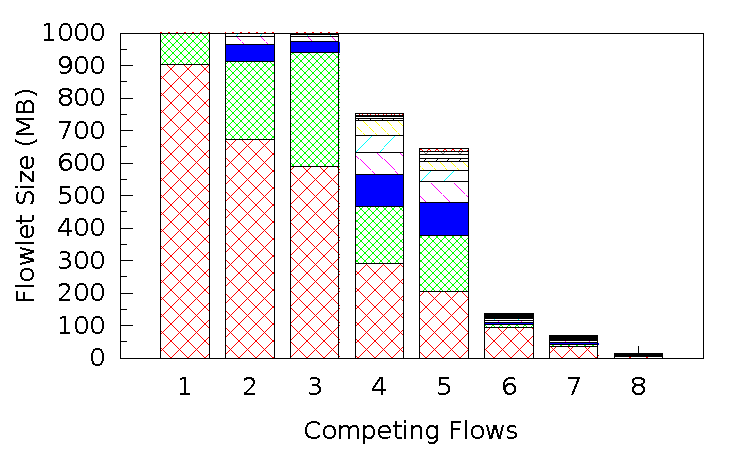
\includegraphics[width=0.7\textwidth]{presto/figures/flowlets/histo.pdf}
        \caption{Stacked histogram of flowlet sizes (in MB) for a 1 GB {\tt scp} file transfer. We vary the number of {\tt nuttcp}~\cite{nuttcp} background flows and
                denote them as {\em Competing Flows}. The size of each flowlet is shown within each bar, and flowlets
                are created whenever there is a 500 $\mu$s delay between segments. The top 10 flowlet sizes are shown here.
                We also analyzed the results of a 1 GB {\tt nuttcp}, {\tt ftp}, and a simple custom client/server transfer and found them
                to be similar. }
        \label{micro_flowlet_size}
\end{figure}

%\aditya{the following two paras don't flow well. they don't make a clear case for why flowlets is a bad idea and TSO segment level switching is a good idea. if reordering is the 100us flowlets' big problem then why not use our receiver-side reordering tricks with 100us flowlets? also it is not clear how were are overcoming reordering simply by relying on TSO segment switching}

%\eric{Rough estimates from our experiments with 100$\mu$s: ~90\% of flowlet sizes are 114KB or less with flowlets. ~00.1\% of flowlets are
%larger than 1 MB, with the largest ranging from 2.1-20.5MB. Some thoughts: (i) 100 $\mu$s flowlets can still have flowlet sizes larger 
%than switch buffers, which can cause congestion/loss when collision occur, (ii) given that flowlet with 100 $\mu$s does not prevent reordering,
%then why should we use flowlets at all? (iii) flowlets were really meant to have inactivity timers larger than the max difference in latency
%over any two paths, and buffer latency at one switch alone is ~4ms, so the use of flowlets on these small time scales is fundamentally
%flawed, (iv) flowlets are sensitive to traffic demand at sender, (v) flowlets are non-uniform in size, (vi) flowlets could break small 
%flows over multiple paths. Using TSO segment ensures: (i) small, uniform units of load-balancing, which means (ii) we are indenpendent
%of traffic demand, (iii) collisions are not a problem b/c TSO size is smaller than buffer size, (iv) most small flows are routed
%over the same path, (v) we do not impose too much computational overhead on sender/receiver and (vi) we still need to solve reordering.}

% Rough outline for next two paragraphs
% Problem with flowlets:
%  1. Sensitive to traffic patterns at the sender
%     a. In practice, we find this means the distribution of flowlet sizes is not uniform, and has a tail
%     b. These tails can still experience hash collisions, albeit less often.
%		i. congestion: lower throughput and to longer mice tail latencies
%  2. Needlessly break down small flows into several flowlets
%     a. Especially early in connection: 100us, 50 KB mice flows broken into 4-5 flowlets
%  3. Designed to be robust to reordering, but difficult to tune
%


Another possibility is to load balance on flowlets~\cite{conga,juniper-vcf}.  
A flow is comprised of a series of bursts, and a flowlet is created when
the inter-arrival time between two packets in a flow exceeds a threshold inactivity timer.  
In practice, inactivity timer values are between 100-500 $\mu$s~\cite{conga}. 
These values intend to strike a good balance between load balancing on a sub-flow level 
and acting as a buffer to limit reordering between flowlets.
Flowlets are derived from traffic patterns at the sender, and in practice this
means the distribution of flowlet sizes is not uniform. To analyze flowlet sizes, a simple experiment is shown in Figure~\ref{micro_flowlet_size}. 
We connect a sender and a receiver to a single switch and start an {\tt scp} transfer designed to 
emulate an elephant flow. Meanwhile, other senders are hooked up to the same switch and
send to the same receiver. We vary the number of these competing flows and show a stacked histogram of 
the top 10 flowlet sizes for a 1 GB {\tt scp} transfer with a 500 $\mu$s inactivity timer. 
The graph shows flowlet sizes can be quite large, with more than half the transfer being attributed
to a single flowlet for up to 3 competing flows. Using a smaller inactivity timer, such 100$\mu$s, helps (90\% of flowlet sizes are 114KB or less), but
does not prevent a long tail: 0.1\% of flowlets are larger than 1 MB, with the largest ranging from 2.1-20.5 MB.
Collisions on large flowlet sizes can lead to congestion.
The second problem with flowlets is that small inactivity thresholds, such as 100 $\mu$s, can lead to significant reordering.
Not only does this impact TCP performance (profiled in Section~\ref{sec:micro}), but it also needlessly 
breaks small flows into several flowlets. With only one flow in the network, we found a 50 KB
mice flow was broken into 4-5 flowlets on average. Small flows typically do not need to be
load balanced on a sub-flow level and need not be exposed to reordering.


%Another possibility is to load balance on flowlets~\cite{conga,juniper-vcf}.  A flow is typically comprised of a series of bursts, and each burst is defined as a flowlet. By monitoring the inter-arrival time of packets in a flow, one can easily define an inactivity timer to seperate flowlets.  In practice, intactivity timer values are between 100-500 $\mu$s~\cite{conga}. These values are intended to strike a good balance between creating enough opportunities to load balance on a sub-flow level and also ensure the reordering is limited at the destination due to the time buffer naturally incurred between flowlets.  We find, however, that it is difficult to strike a balance between achieving fine-grained, near-optimal load balancing and robustness against reordering. We perform a simple experiment in Figure~\ref{micro_flowlet_size}.  We connect a sender and a receiver to a single switch and start a transfer over an application designed to emulate an elephant flow ({\tt scp}). Meanwhile, we also hook up other senders to the same switch and have them send to the same reciever. We vary the number of competing flows and show a stacked histogram of the top 10 flowlet sizes for a 1 GB scp transfer with a 500 $\mu$s inactivity timer. \eric{Competing flows use nuttcp.} The graph shows flowlet sizes can be large, which means hash collisions can still occur on large flowlets.  Using a smaller timeout, such as 100 $\mu$s, creates smaller flowlets, but as we show in Section XXX, suffers from severe reordering that greatly reduces throughput and hurts applications.  \eric{mention creates congestion, which leads to lower thorughput and increase mice FCT latency}

% What do we want in sub-flow load balancing?
%  A. Want to move toward idealized ECMP: uniform sub-flow load balancing without the tail
%  B. Units should be as small as possible for fine-grained load balancing, but
%       not so small to be inefficient (TSO) or break small flows into parts
%  C. Independent of traffic patterns on sender
%  As a result, we settle on...

The shortcomings of the previous approaches lead us to reconsider on what granularity
load balancing should occur. 
%We take motivation from a best-case ECMP scenario. 
Ideally, sub-flow load balancing should be done on near uniform sizes.
%independent of traffic patterns on the sender to avoid long tails. 
Also, the unit of load balancing should be small to
allow for fine-grained load balancing, but not so small as to break small flows into 
many pieces or as to be a significant computational burden. As a result, we
propose load balancing on 64 KB units of data we call {\em flowcells}. Flowcells
have a number of advantages. First, the maximum segment size supported by TSO
is 64 KB, so flowcells provide a natural interface to high speed optimizations provided
by the NIC and OS and can scale to fast networking speeds. Second, an overwhelming fraction of mice flows are less than 64 KB in size
 and thus do not have to worry about reordering~\cite{benson10,vl2,kandula2009nature}.
Last, since most bytes in datacenter networks originate from elephant flows~\cite{kandula2009nature,benson10,dctcp},
this ensures that a significant portion of datacenter traffic is routed on uniform
sizes. While promising, this approach must combat reordering to be effective. 
Essentially we make a trade-off: 
%we provide line rate load balancing in the most effective
%manner as to avoid congestion and then handle reordering head-on at the receiver.
the sender avoids congestion by providing fine-grained, near-uniform load balancing,
and the receiver handles reordering to maintain line-rate.


%We highlight the challenges of this approach
%in the next subsection and provide a design to mitigate reordering problems in Section~\ref{sec:design}.

%In order to obtain fine-grained, near-optimal load balancing, we should stripe on a granularity
%that is indendpent of traffic patterns, near-uniform in size, and as small as possible while still
%scaling to fast network speeds.
%Therefore, we argue the TSO segment~\keqiang{what about saying maximum TSO segment size (64KB), each TSO segment's size is bounded by maximum TSO size} 
%is the natural granularity in which to load balance. Doing so
%provides several benefits. First, TSO segments are small and near-uniform in size, so an
%effective load-balancing scheme should be able to closely track the optimal case of per-packet
%load balancing, but without the additional computational overhead.
%Second, the TSO engine in the NIC will ensure that all packets created from a TSO segment will contain the same
%header information. We show in Section XXX how this is important to deal with reordering because
%we can easily impart metadata on all packets within a segment that help us distinguish loss from 
%ordering~\keqiang{all the packets within the same flowcell contain the same flowcell id.  
%"all packets created from a TSO segment will contain the same
%header information" is fine but a flowcell can contrain several TSO segments depending on TSO segment size}.
%Last, small flows less than 64 KB in size will actually be routed over the
%same path in the network, meaning a very large fraction of mice flows will not be routed on a subflow
%level and thus do not have to worry about reordering~\cite{benson10,vl2,kandula2009nature}~\keqiang{Around 90\% of datacenter flows' sizes are smaller than 64KB~\cite{benson10}, 
%meaning the overwhelming majority is load balanced like ECMP and we only need to engineering the left 10\%}.
%\eric{need to mention that we can combine segments as long as not above 64 KB, so not really
%per TSO segment. helps in small flows.}
%While promising, this approach has a major challenge: reordering. We highlight these challenges
%in the next subsection and provide a design to mitigate the problems in Section~\ref{sec:design}.

\tightparagraph{Per-Hop vs End-to-End Multipathing}
The last design consideration is whether multipathing should be done on a local, per-hop level (\eg{}ECMP), or
on a global, end-to-end level. In Presto, we choose the latter: pre-configured end-to-end paths
are allocated in the network and path selection (and thus multipathing) is realized by having the network edge
place flowcells onto these paths. 
Presto can be used to load-balance in an ECMP style per-hop manner, but the choice of end-to-end 
multipathing provides additional benefits due to greater control of how flowcells are mapped to
paths. Per-hop multipathing can be inefficient
under asymmetric topologies~\cite{wcmp}, and load-balancing on a global end-to-end level can allow
for weighted scheduling at the vSwitch to rebalance traffic. This is especially important when failure occurs.
The second benefit is flowcells can be assigned over multiple paths very evenly
by iterating over paths in a round-robin, rather than randomized, fashion. 

%As we show
%in Section~\ref{sec:micro}, randomization in per-hop multipathing can lead to "unluckiness" where
%multiple flowcells get sent to the same link over a small timescale by multiple flows. This transient congestion
%can lead to increased buffer occupancy and higher delays in the network. These benefits can
%fundamentally be provided at the per-hop level (\cite{wcmp} handles asymmetry), but require changes to networking firmware. 
%These considerations motivate us to utilize end-to-end multipathing, but Presto can also
%use per-hop multipathing when conveinent.

\subsection{Reordering Challenges}
%The above design decisions in Presto cause following main challenges:
Due to the impact of fine-grained, flowcell-based load balancing, Presto must account for reordering. Here, we 
highlight reordering challenges. The next section shows how Presto deals with these concerns.

%\tightparagraph{Soft Edge Distributed Load Balancing}
%There are two main challenges in implementing load balancing at the soft edge. First, the implementation
%must scale to fast networking speeds because networking at 10+ Gbps can have significant overhead if not carefully
%considered. Therefore, in order to achieve line rate, great care must be taken to ensure that load balancing
%schemes are light-weight, simple and can take advantage of optimizations provided by the NIC and OS.  
%The second major problem is how to load balance in a distributed fashion at the vSwitches in such
%a way that the load balancing performs well globally.
%Nodes must ensure they are spreading
%their traffic equally throughout the network, but in a low-overhead fashion that does not require detailed
%topographical information about the network, real-time traffic matrices, or strict coordination
%with other senders.

%\eric{several things to add: in presto, we can just make dumb edge decisions and not have to worry
%about (i) the traffic patterns, that is who else is sending, (ii) topology asymmetry. Basically,
%we want to highight that the vSwitch shouldn't require a lot of detailed network-wide information,
%but should be able to somehow still load balance in a way that performs very well globally.}

\tightparagraph{Reordering's Impact on TCP} The impact of reordering on TCP is well-studied~\cite{leung2007overview,paxson1997end}. 
Duplicate acknowledgments caused by reordering
can cause TCP to move to a more conservative sender state and reduce the sender's congestion window.
Relying on parameter tuning, such as adjusting the DUP-ACK threshold, is not ideal because 
increasing the DUP-ACK threshold increases the time to recover from real loss. Other TCP settings
such as Forward Acknowledgement (FACK) assume un-acked bytes in the SACK are lost and degrade
performance under reordering. 
A scheme that introduces reordering should not rely on careful configuration of TCP parameters
because (i) it is hard to find a single set of parameters that work effectively over multiple 
scenarios and (ii) datacenter tenants should not be forced to constantly tune their networking stacks.
Finally, many reordering-robust variants of TCP have been proposed~\cite{rr-tcp,blanton2002making,tcp-pr}, but
as we will show, GRO becomes ineffective under reordering. Therefore, reordering should
be handled below the transport layer.

\tightparagraph{Computational Bottleneck of Reordering}
Akin to TSO, Generic Receive Offload (GRO) mitigates the computational burden of receiving
1500 byte packets at 10 Gbps. GRO is implemented in the kernel of the hypervisor,
and its handler is called directly by the NIC driver. It is responsible
for aggregating packets into larger segments that are pushed up to OVS and the TCP/IP stack. 
GRO is implemented in the Linux kernel and is used even without virtualization. Similar
functionality can be found in Windows (RSC~\cite{ms-rsc}) and hardware (LRO~\cite{grossman2005large}).

Because modern CPUs use aggressive prefetching, the cost of receiving
TCP data is now dominated by per-packet, rather than per-byte, operations.
As shown by Menon~\cite{optimize-tcp-receive},  the majority of this overhead comes from
buffer management and other routines not related to protocol processing, and therefore 
significant computational overhead can be avoided by aggregating "raw" packets from
the NIC into a single {\tt sk\_buff}.
%\footnote{Refer to~\cite{linuxgro,optimize-tcp-receive} for detailed study and explanation}
Essentially, spending a few cycles to aggregate packets within GRO creates less segments for
TCP and prevents having to use substantially more cycles at higher layers in the networking stack.
Refer to~\cite{linuxgro,optimize-tcp-receive} for detailed study and explanation.

To better understand the problems reordering causes, a brief description of  
the TCP receive chain in Linux follows. First, interrupt coalescing allows the NIC to create an interrupt for a batch of packets~\cite{mogul1997eliminating,understanding-linux-network},
which prompts the driver to poll the packets into an aggregation queue. Next, the driver
invokes the GRO handler, located in the kernel, which
{\em merges} the packets into larger segments. The merging continues,
possibly across many polling events, until a segment
reaches a threshold size, a certain age, or cannot be combined with the incoming packet. Then, the
combined, larger segment is {\em pushed up} to the rest of the TCP/IP networking stack. The GRO process is
done on a per-flow level. With GRO disabled, throughput drops to around
5.7-7.1 Gbps and CPU utilization spikes to 100\% (Section~\ref{sec:micro} and~\cite{bullettrains}). 
Receive offload algorithms, whether in hardware (LRO)~\cite{grossman2005large,open-lro} or in software (GRO), are usually
{\em stateless} to make them fast: no state is kept beyond the segment being merged.


%\begin{figure}[!htb]
%        \centering
%  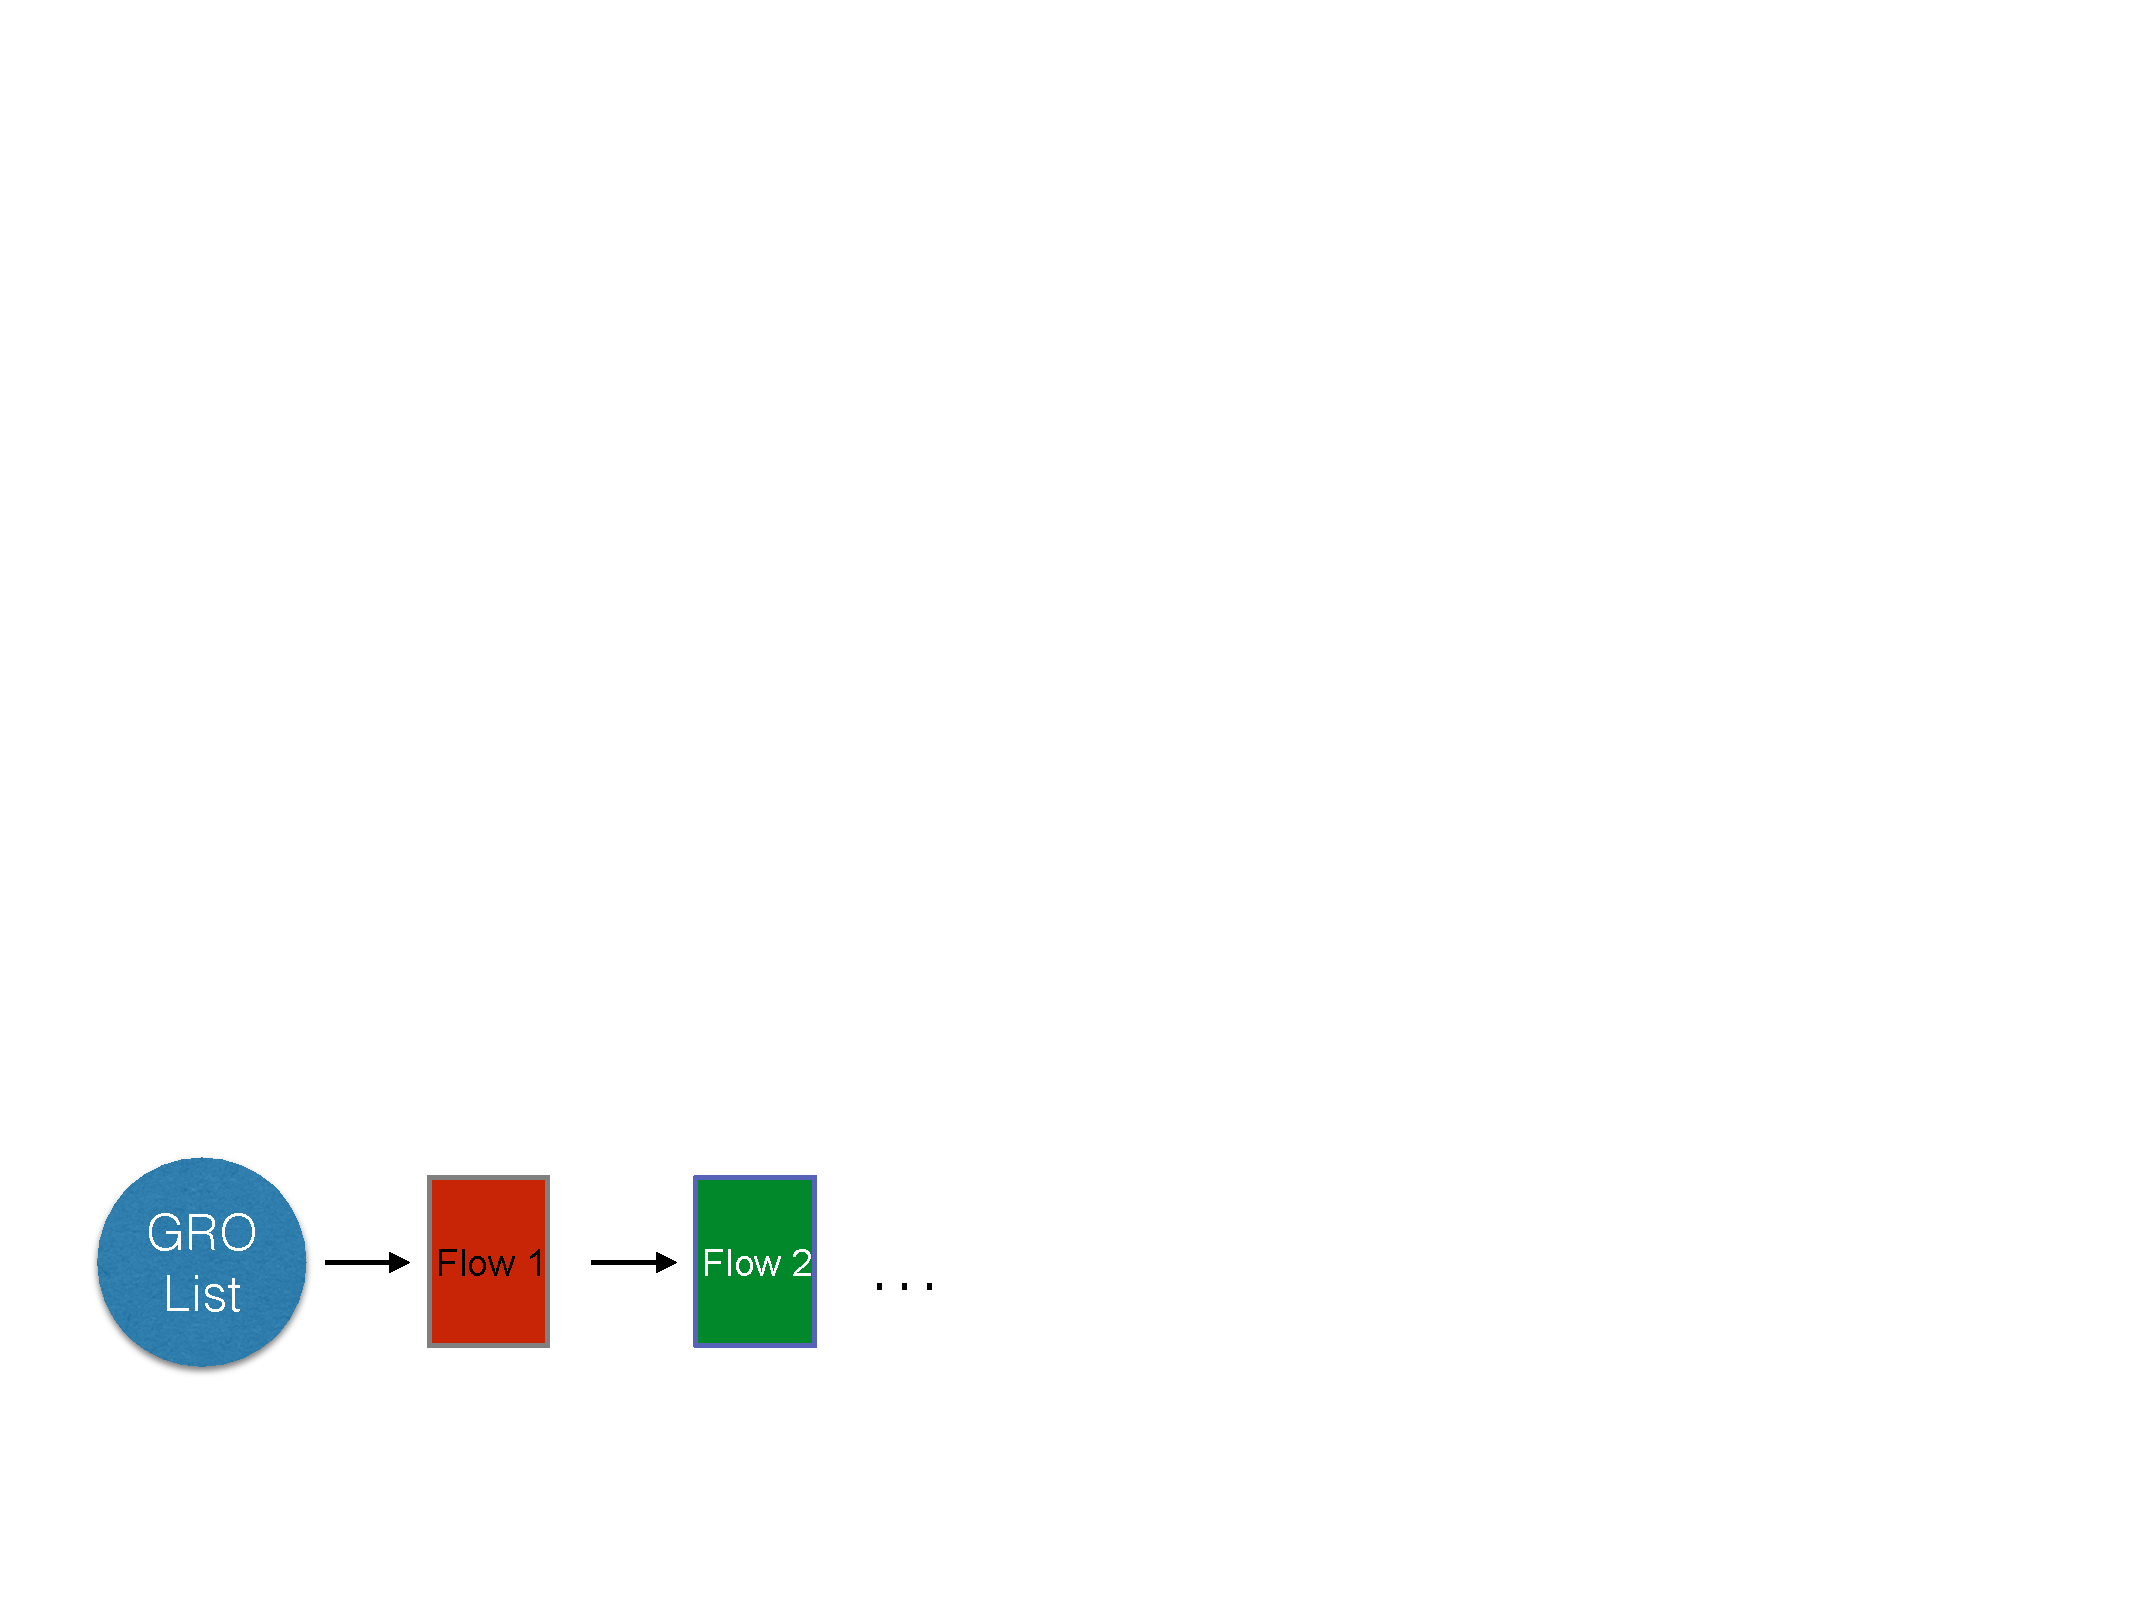
\includegraphics[width=0.45\textwidth]{presto/figures/gro-design/gro.pdf}
%        \caption{GRO design. FIX ME!}
%        \label{gro-design}
%\end{figure}

\begin{figure}[!t]
        \centering
  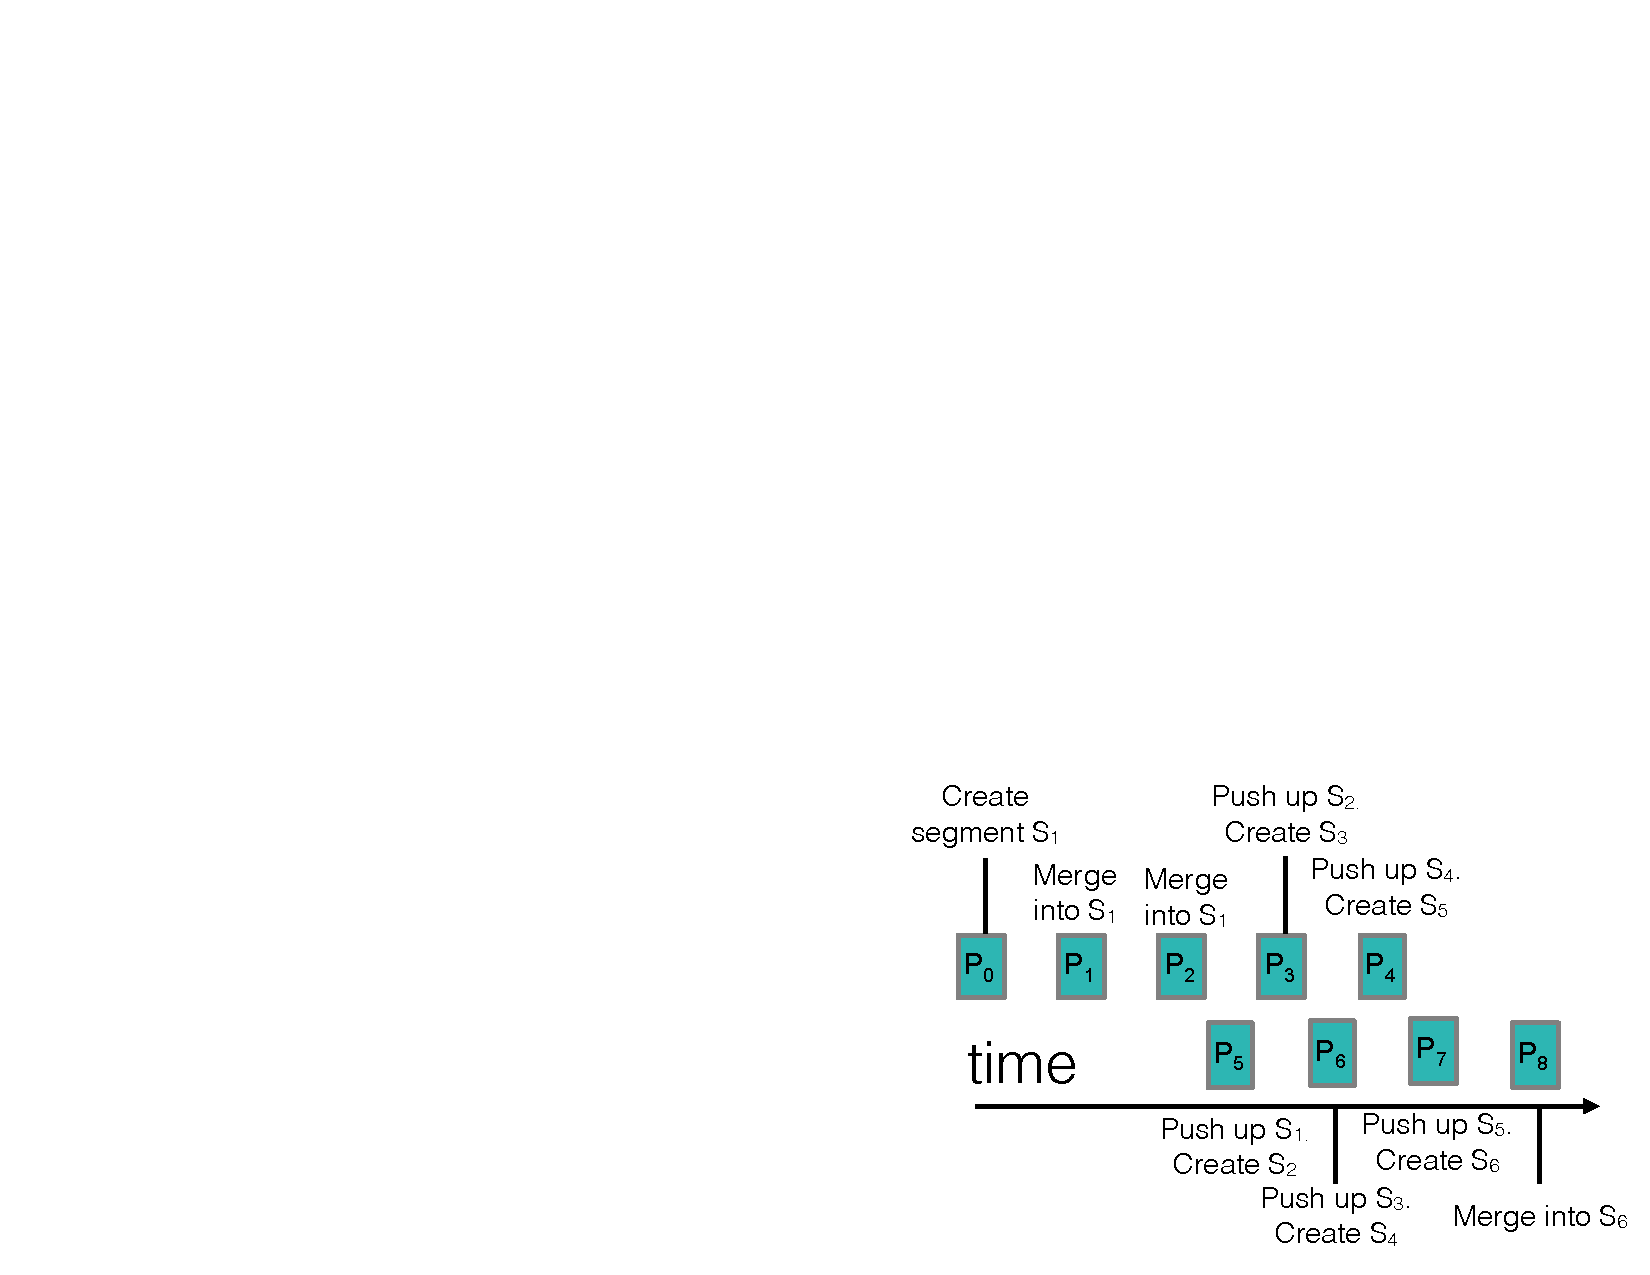
\includegraphics[width=0.7\textwidth]{presto/figures/gro-design/gro-break.pdf}
        \caption{GRO pushes up small segments ($S_i$) during reordering.}
        \label{gro-break}
\end{figure}


We now uncover how GRO breaks down in the face of reordering. Figure~\ref{gro-break} shows the impact of reordering on GRO.  Reordering does not allow the segment to grow: each reordered packet cannot be merged with the existing segment, and thus the previously created segment must be pushed up. With extreme reordering, GRO is effectively disabled because small MTU-sized segments are constantly pushed up. This causes (i) severe computational overhead and (ii) TCP to be exposed to significant amounts of reordering. We term this the {\em small segment flooding} problem.

Determining where to combat the reordering problem has not previously taken the small segment flooding problem into account.  Using a reordering buffer to deal with reordered packets is a common solution (\eg{}works like~\cite{drb} re-sort out-of-order packets in a shim layer below TCP), but a buffer implemented above GRO cannot prevent small segment flooding.  Implementing a buffer below GRO means that the NIC must be changed, which is (i) expensive and cumbersome to update and (ii) unlikely to help combat reordering over multiple interrupts.

In our system, the buffer is implemented in the GRO layer itself.  We argue this is a natural location because GRO can
directly control segment sizes while simultaneously limiting the impact of reordering. 
Furthermore, GRO can still be applied on packets pushed up from LRO, which means hardware doesn't have to be modified
or made complex.
Implementing a better GRO algorithm has multiple challenges. The algorithm should be light-weight to scale to fast networking speeds. Furthermore, an ideal scheme should be able to distinguish loss from reordering.  When a gap in sequence numbers is detected (\eg{}when $P_5$ is received after $P_2$ in Figure~\ref{gro-break}), it is not obvious if this gap is caused from loss or reordering.  If the gap is due to reordering, GRO should not push segments up in order to try to wait to receive the missing gap and merge the missing packets into a preestablished segment.  If the gap is due to loss, however, then GRO should immediately push up the segments to allow TCP to react to the loss as fast as possible. Ideally, an updated GRO algorithm should ensure TCP does not perform any worse than a scheme with no reordering. Finally, the scheme should adapt to prevailing network conditions, traffic patterns and application demands.




\section{Design}
\label{rate-limiter:sec:design}

\subsection{Direct ECE Marking}
\begin{algorithm}[!t]
\caption{Pseudo-code of Direct ECE Marking Algorithm}
\label{alg:algorithm1}
\begin{algorithmic}[1]
\FOR{each incoming TCP ACK p}
\STATE q $\leftarrow$ rate\_limiter\_queue(p)
\IF{len(q) $>$ {\emph {K}}}
\STATE tcp(p).ece $\leftarrow$ 1
\ENDIF
\ENDFOR
\end{algorithmic}
\end{algorithm}

In this subsection, we introduce a technique called Direct ECE Marking (DEM). 
DEM assumes that VMs and containers are configured with DCTCP congestion control algorithm. 
In~\dem{}, we monitor rate limiter queue occupancy and process each incoming TCP ACK. 
If the current rate limiter queue occupancy is above a threshold $K$, 
we directly set the ACK's TCP ECE (ECN Echo) bit to 1.
To get the correct rate limiter queue occupancy for the TCP ACK, we need to inspect the TCP ACK and
determine which queue the incoming TCP ACK's data packet belongs to. In other words, we need to 
determine the queue that this TCP ACK's reverse flow goes to.
The pseudo-code of~\dem{} is presented in Algorithm~\ref{alg:algorithm1}.~\dem{} can be
implemented in the virtual switch (e.g., OVS) in the hypervisor. OVS rate limiters directly call
the Linux HTB implementation so it can get the rate limiter queue information. Also, OVS processes all the packets
so it can inspect and modify all the incoming TCP ACKs. 

The difference between~\dem{} 
and existing ECN marking schemes is that it directly marks TCP ECE bit based on 
current queue occupancy instead of the queue occupancy one TCP RTT ago if using the existing ECN marking schemes.
Therefore, congestion control actions depend on real-time queueing information and control loop latency 
is reduced to almost 0. Control loop latency is the time it takes to forward the TCP ACK from the 
virtual switch to the VM or container. In this way, ``in network'' latency does not cause 
side-effects for end-host congestion control. Note that if we perform ECN marking on the outgoing path, then 
congestion control loop latency can be very large (e.g., RTT of the flows to remote clients is tens of ms).
Besides reducing control loop latency,~\dem{} also avoids coarse-grained segment-level ECN marking, 
which leads to inaccurate congestion level estimation, as we discussed before.
Therefore,~\dem{} makes rate limiter congestion control more timely and effective.

DEM only turns TCP ECE bit from 0 to 1, it never does the opposite. 
If congestion happens both in the rate 
limiter on the end-host and in the switch(es) on the network path, Then TCP ECE bit is always 1. 
If congestion only happens
in the rate limiter, then~\dem{} turns TCP ECE bit from 0 to 1. 
If congestion only happens in the network (i.e., in the switches), then TCP ECE is kept as 1.
If neither network switches nor the rate limiter is congested, then TCP ECE is always 0.
So~\dem{} does not affect the correctness of end-to-end
congestion control and is complementary with ``in network'' congestion control schemes.

\iffalse
\subsection{~\spring{}}

\begin{algorithm}[!t]
\caption{Pseudo-code of~\spring{} Algorithm}
\label{alg:algorithm3}
\begin{algorithmic}[1]
\FOR{each packet p}
\STATE q $\leftarrow$ rate\_limiter\_queue(p)
\STATE current\_qlen $\leftarrow$ len(q)
\STATE new\_gradient $\leftarrow$ current\_qlen -- q.prev\_qlen
\STATE q.prev\_qlen $\leftarrow$ current\_qlen
\STATE q.gradient $\leftarrow$ (1 -- $\alpha$)*q.gradient + $\alpha$*new\_gradient
\STATE q.normalized\_gradient $\leftarrow$ q.gradient / {\emph {K1}}
\IF{p is an incoming TCP ACK}
\STATE f $\leftarrow$ getReverseFlow(p)
\IF {current\_qlen $<$ {\emph {K1}}}
\STATE f.rwnd $\leftarrow$ f.rwnd + MSS
\ELSIF {current\_qlen $>$ {\emph {K2}}}
\STATE f.ssthresh $\leftarrow$ f.rwnd
\STATE f.rwnd $\leftarrow$ f.rwnd*(1 -- $\beta$*(1 -- $\frac{current\_qlen}{K2}$))
\STATE f.rwnd $\leftarrow$ min(f.rwnd, MSS)
\ELSIF {q.gradient $\le$ 0}
\STATE f.rwnd $\leftarrow$ f.rwnd + MSS
\ELSE
\STATE f.rwnd $\leftarrow$ f.rwnd*(1 -- $\beta$*q.normalized\_gradient)
\STATE f.rwnd $\leftarrow$ min(f.rwnd, MSS)
\ENDIF
\ENDIF
\ENDFOR
\end{algorithmic}
\end{algorithm}

DEM has two limitations. First is that it relies on 
DCTCP transport in VMs and containers. For containers, cloud administrators are able to configure
server's congestion control algorithm to DCTCP. So such an assumption is reasonable. 
However, for VMs, tenants have the flexibility to tune their congestion control settings.
Therefore, assuming that every VM uses DCTCP as the congestion control algorithm is not realistic in practice.
Second,~\dem{} needs ECN support in the network. As mentioned before, 
ECN is not widely supported in WAN traffic~\cite{kuhlewind2013state}.
To address the limitations and make our solution more generic, we present~\spring{} (shown in Algorithm~\ref{alg:algorithm3}).

~\spring{} modifies TCP ACK's receiver's 
advertised window size (RWND) to enforce congestion control~\cite{he2016ac,cronkite2016virtualized}.
It uses real-time rate limiter queue length as congestion control signal and 
a TIMELY-like~\cite{mittal2015timely} congestion control law.
For each packet, 
we get its corresponding rate limiter queue length.
If the packet is outgoing, we get the length of the queue that the packet is to be enqueued.
If the packet is an incoming TCP ACK, we get the length of the queue that 
its reverse flow goes to (TCP is bidirectional).  
We maintain a gradient for the rate limiter queue length using 
Exponentially Weighted Moving Average (EWMA) (line 2--6). 
We set two thresholds, $K1$ and $K2$ ($K1 < K2$). The queue length gradient is normalized by dividing it using $K1$ (line 7).
Note that gradient is a per-queue defined parameter.
If the processed packet is an incoming TCP ACK, we first need to get its reverse 
flow (i.e., the TCP ACK's corresponding data packet flow). Then, 
we manage a running RWND for each flow based on a TIMELY-like congestion control law 
(line 10-- line 20). There are 4 cases: 
if the current rate limiter queue length is smaller than $K1$, that means this is no congestion, so we 
increase the flow's RWND by one MSS (Maximum Segment Size). If the current rate limiter queue length is larger
than $K2$, that means congestion happens in the rate limiter queue, so we multiplicatively decrease the RWND. 
If the current rate limiter queue length is between $K1$ and $K2$, we check the gradient of rate limiter queue occupancy.
If the gradient is smaller than or equal to 0, that means the queue is being drained or its size is not increasing, we 
increase RWND by one MSS. Otherwise, we multiplicatively decrease the RWND based on the normalized gradient.

Note that TIMELY~\cite{mittal2015timely} is a rate-based congestion control algorithm while~\spring{} is a window-based.
TIMELY uses accurate latency measurement provided by the NIC while~\spring{} performs congestion control based on 
real-time rate limiter queue length. Because congestion control decisions are enforced via modifying RWND field in TCP ACK headers,~\spring{} has the following good properties: 
1) the solution does not relies on DCTCP transport in VMs and ECN support in the network, 
so it is generic and can support not only east-west traffic (i.e., intra-datacenter traffic) but also north-south traffic
(i.e., inter-datacenter traffic and traffic between cloud and clients). 
2) the solution avoids coarse-grained segment-level ECN marking and its control loop latency is almost 0, so congestion control
is more effective compared with the strawman solution---DCTCP in VMs/containers and ECN marking in rate limiter queues.  

\subsection{Remarks}
Both~\dem{} and~\spring{} avoid long and unpredictable congestion control loop latency and avoid throughput oscillation due to 
coarse-grained segment-level ECN marking.~\dem{} relies on ECN support in the network and DCTCP transports configured in
the end-points. Compared with~\dem{},~\spring{} is a more generic solution.~\dem{} and~\spring{} share the same limitation, that is
they do not support IPSec (because they need to modify TCP header). However, SSL/TLS is supported. 
Furthermore,~\spring{} needs to maintain per-flow information in the hypervisor. 
Maintaining per-flow information in switches is conventionally considered to be challenging.
In~\spring{} we only need to maintain the information of the connections from the VMs/Containers running on the end-host. 
Also, recent advances like OVS ConnTrack~\cite{ovs-conntrack} has made connection tracking on the end-host more effective.

\fi 

\section{Implementation}
\label{impl}
This section outlines relevant implementation details.~\acdc{} was implemented 
in Open vSwitch (OVS) v2.3.2~\cite{ovs-website} and
about 1200 lines of code (many are debug/comments) were added. 
A high-level overview follows.
\crs{
A hash table is added to OVS, and flows are hashed on a 5-tuple (IP addresses, ports and VLAN) to obtain a flow's state.
The flow entry state is 320 bytes and is used to maintain the congestion control state mentioned in \sref{design}.
SYN packets are used to create flow entries, and FIN packets, coupled with a course-grained garbage
collector, are used to remove flow entries. Other TCP packets, such as data and ACKs, trigger 
updates to flow entries.
There are many more table lookup operations (to update flow state)
than table insertions or deletions (to add/remove flows). Thus, Read-Copy-Update (RCU)
hash tables~\cite{guniguntala2008read} are used to enable efficient lookups.
Additionally, individual {{\tt spinlocks}} are used on each flow entry in order to allow
for multiple flow entries to be updated simultaneously.
}

\crs{
Putting it together, the high-level operation on a data packet is as follows. An application on the sender generates a packet
that is pushed down the network stack to OVS. The packet is intercepted in 
the function {\tt  ovs\_dp\_process\_packet}, where the
packet's flow entry is obtained from the hash table. Sequence number state is updated in the flow entry and ECN bits are set on
the packet if needed (see \sref{design}).
If the packet's header changes, the IP checksum is recalculated. Note TCP checksumming is offloaded to the NIC.
The packet is sent over the wire and received at the receiver's OVS. The receiver updates congestion-related state, strips
off ECN bits, recomputes the IP checksum, and pushes the packet up the stack. ACKs eventually triggered by the packet
are intercepted, where the congestion information is added. Once the ACK reaches the sender, the~\acdc{} module uses
the congestion information to compute a new congestion window. Then it modifies~\rwnd{} with a {{\tt memcpy}}, 
strips off ECN feedback and recomputes the IP checksum before pushing the packet up the stack.
Since TCP connections are bi-directional, two flow entries are maintained for each connection. 
}

\crs{
Our experiments in~\sref{micro} show the CPU overhead of~\acdc{} is small and several implementation details
help reduce computational overhead. First, OVS sits 
above NIC offloading features (\ie{}TSO and GRO/LRO) in the networking stack. Briefly, NIC offloads allow 
the host to pass large data segments along the TCP/IP stack and only deal with MTU-sized packets in the NIC. Thus,~\acdc{}
operates on a segment, rather than a per-packet, basis. Second, 
congestion control is a relatively simple algorithm, and thus the computational burden is not high. Finally,
while~\acdc{} is implemented in software, it may be possible to further reduce the
overhead with a NIC implementation. Today, "smart-NICs"
implement OVS-offload functionality~\cite{cavium-nic,netronome-nic},  
naturally providing a mechanism to reduce overhead and support hypervisor bypass (\eg{}SR-IOV). 
}
%We have also considered designing an~\acdc{}-enabled middlebox to support
%legacy systems that do not run OVS and cannot upgrade their NICs.


%
%Standard OVS kernel datapath LoC: 2360
%\acdc{} kernel datapath LoC: 3590
%
%\tightparagraph{UDP traffic} How to handle.
%Mention VxLAN traffic too.
%\keqiang{and IPsec}
%
%\tightparagraph{No vSwitch}
%\keqiang{title should be hypervisor-bypass?}
%Use middleboxes (for DB server).
%Use NIC (for SR-IOV).
%Hypervisor bypass (e.g., SR-IOV), where TCP traffic is sent to the NIC directly without
%going through hypervisor. First, as noted by~\cite{shieh2011sharing}, ``loss of the security and
%manageability features provided by the software virtual switch has limited
%the deployment of direct I/O NICs in public clouds''. Second, based on techniques like Intel
%DPDK~\cite{intel-dpdk} and ``smart NICs''~\cite{cavium-nic,netronome-nic}, we believe that low latency
%congestion control enforcement schemes like \acdc{} can also be
%employed for hypervisor bypass use cases.
%We need to worry about legacy systems and non-VM systems. For instance, a database or storage device that may not have OVS installed on it.
%We need to talk about either a middlebox or that this percentage of traffic is low? Or implement in NIC (especially one with OVS offload?).
%
%
%\tightparagraph{Little CPU and memory overhead}
%In our implementation, first we leverage the Read-Copy-Update (RCU)~\cite{guniguntala2008read} enabled hash tables
%to keep per-flow states (such as ``snd\_una'' and ``snd\_nxt''). RCU technique is also employed by
%Open vSwitch's kernel datapath and it helps improve processing speed for ``read-heavy''
%workloads (\ie{}, inserting new flows is much less frequent than looking-up existing flows) on
%shared-memory multiprocessor systems.
%Second, \acdc{} processes on ``segment'' level instead of ``packet'' level due to
%NIC offloading features (TSO at the sender side and GRO/LRO at the receiver side).
%Third, we also leverage the NIC checksumming offloading feature such that
%we do not need to compute checksums after we change TCP/IP header fields.
%Our microbenchmarks (\cref{micro}) show that \acdc{} incurs very little additional CPU overhead (less than 4\%) to
%support 10Gbps line-rate, even it is fully implemented in software.
%We are currently implementing \acdc{} on Cavium's programmable NICs~\cite{cavium-nic},
%where we can entirely offload the computational overhead to hardware. Therefore, we believe
%\acdc{} can support even higher line rates (\eg{}, 40Gbps).
%In our implementation, each TCP connection takes 320 bytes in the hash tables,
%so it takes around 3.2MB even there are 10K concurrent connections.
%{~\keqiang{i think we may want to mention that we use both FACK and PACK because we want to be compatible with TSO and try to minimize the CPU/traffic overhead.}

\section{Results}
\label{results}
This section quantifies
the effects of~\acdc{} and determines if the performance of DCTCP
implemented in the vSwitch (\ie{}, \acdc{}) is equivalent to
the performance of DCTCP implemented in the host TCP stack.

\tightparagraph{Testbed}
The experiments are conducted on a physical testbed with 17 
IBM System x3620 M3 servers (6-core Intel Xeon
2.53GHz CPUs, 60GB memory) and Mellanox ConnectX-2 EN 10GbE NICs.
Our switches are IBM G8264, each with a buffer of 9MB shared
by forty-eight 10G ports. 
%The switches have dynamic memory management enabled by default.

\tightparagraph{System settings}
We run Linux kernel 3.18.0 which implements DCTCP as a 
pluggable module.
We set {{\tt $RTO_{min}$} to 10 ms~\cite{vasudevan2009safe,judd2015nsdi} and
set parameters {\tt tcp\_no\_metrics\_save}, {\tt tcp\_sack} and {\tt tcp\_low\_latency} to 1.
\crs{Results are obtained with MTU sizes of 1.5KB and 9KB,
as networks typically use one of these settings. 
Due to space constraints, a subset of
the results are presented and unless otherwise noted, the MTU is set to 9KB.}



\tightparagraph{Experiment details}
To understand~\acdc{} performance, three different congestion control configurations
are considered. The baseline scheme, referred to as {\em CUBIC}, configures
the host TCP stack as CUBIC (Linux's default congestion control), which runs on top of an unmodified version of OVS.
Our goal is to be similar to {\em DCTCP}, which configures the host TCP
stack as DCTCP and runs on top of an unmodified version of OVS. Our scheme,{\em ~\acdc{}},
configures the host TCP stack as CUBIC (unless otherwise stated) and implements DCTCP congestion control in OVS.
In DCTCP and~\acdc{}, WRED/ECN is configured on the switches. In CUBIC,
WRED/ECN is not configured.

The metrics used are: TCP RTT (measured by sockperf~\cite{sockperf}),
TCP throughput (measured by iperf),
loss rate (by collecting switch counters) and
Jain's fairness index~\cite{jain-index}.
In \sref{macro}, flow completion time (FCT)~\cite{dukkipati2006flow} is used 
to quantify application performance.~\crs{All benchmark tools are run
in a container on each server, rather than in a VM.}

\subsection{Microbenchmarks}
\label{micro}
\begin{figure}[!t]
        \centering
        \begin{subfigure}[b]{0.45\textwidth}
                \centering
                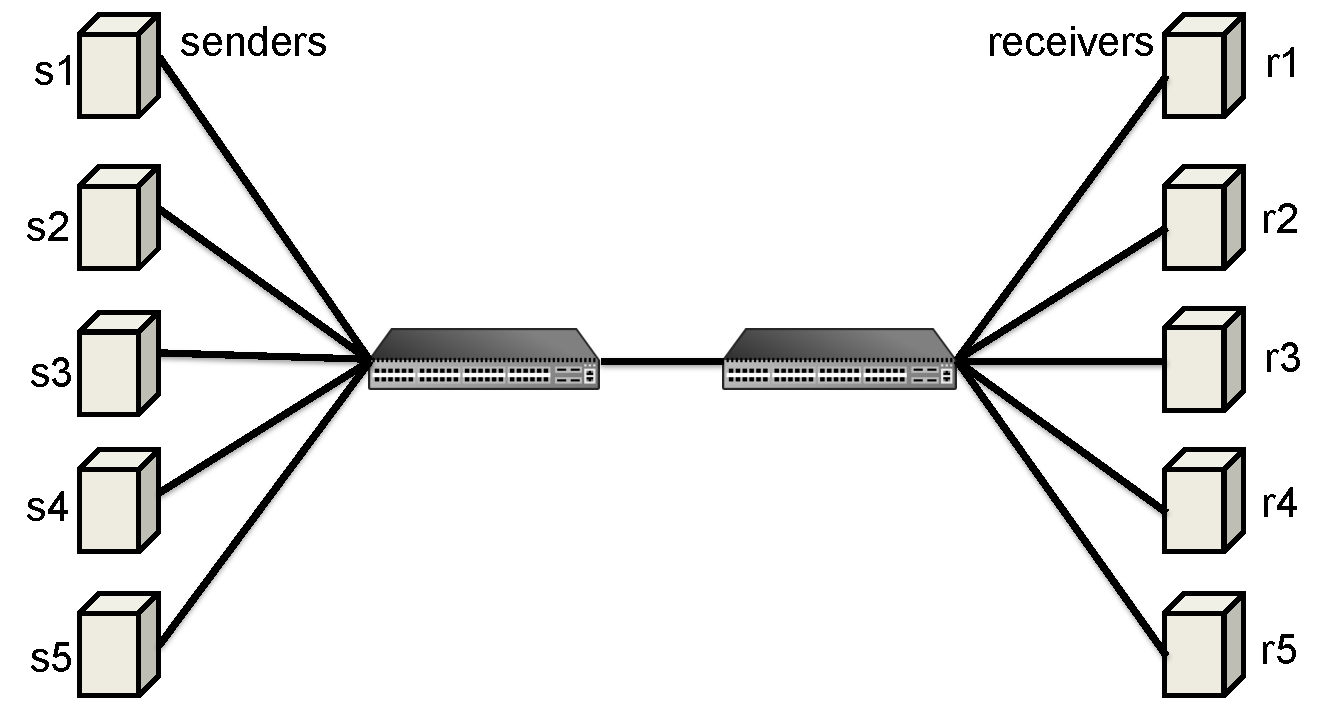
\includegraphics[width=0.7\textwidth]{acdctcp/figures/dumbbell_topology.pdf}
                \caption{Dumbbell topology.}
                \label{dumbbell_topology}
        \end{subfigure}
        \begin{subfigure}[b]{0.45\textwidth}
                \centering
                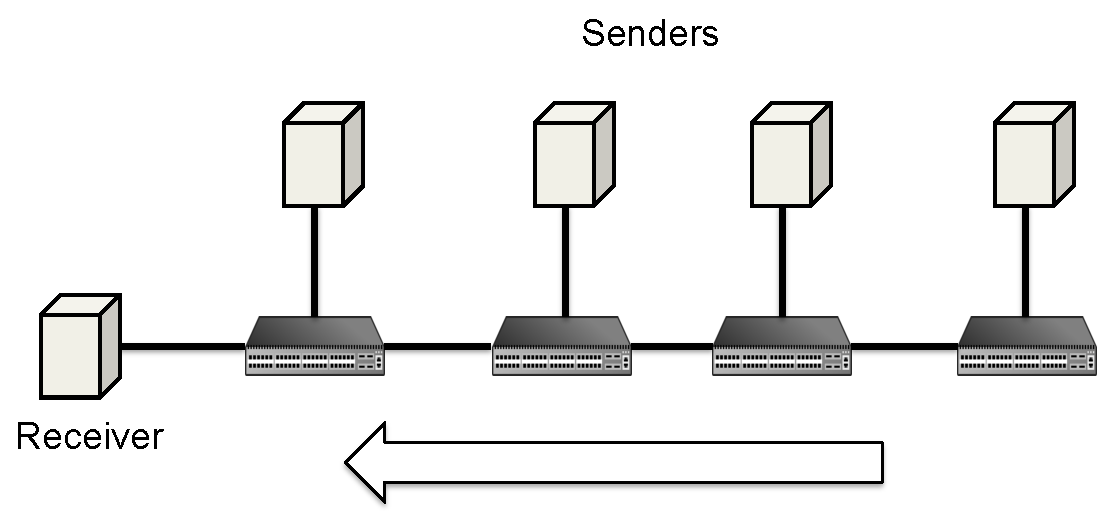
\includegraphics[width=0.7\textwidth]{acdctcp/figures/parkinglot_topology.pdf}
                \caption{Multi-hop, multi-bottleneck (parking lot) topology.}
                \label{parkinglot_topology}
        \end{subfigure}
        \caption{Experiment topologies.}
        \label{microbenchmarks_topology}
\end{figure}

%%%% topology %%%

\begin{figure}[!t]
        \centering
  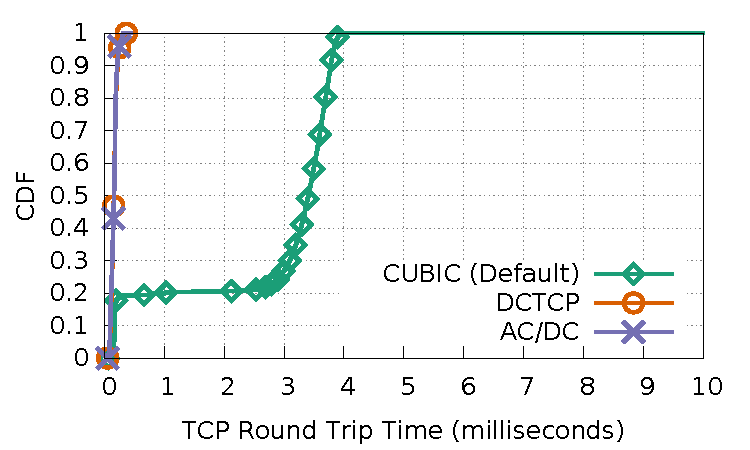
\includegraphics[width=0.5\textwidth]{acdctcp/figures/convergence/flowcontrolOFF_sockperf/convergence_test_sockperf.pdf}
        \caption{RTT of schemes on dumbbell topology.}
        \label{sockperf_convergence}
\end{figure}

We first evaluate \acdc{}'s performance using a set of microbenchmarks.
The microbenchmarks are conducted on topologies shown in Figure~\ref{microbenchmarks_topology}.

\tightparagraph{Canonical topologies}
We aim to understand the performance of our scheme on two simple topologies.
First, one long-lived flow is started per server pair ($s_i$ to $r_i$) in Figure~\ref{dumbbell_topology}. 
The average per-flow throughput of \acdc{}, DCTCP and CUBIC are all 1.98Gbps.
Figure~\ref{sockperf_convergence} is a CDF of the RTT
from the same test. Here, increases in RTT are caused by queueing delay in the switch.
~\acdc{} achieves comparable RTT with DCTCP and significantly outperforms CUBIC.

Second, each sender in Figure~\ref{parkinglot_topology} starts a long-lived
flow to the receiver. Each flow traverses a different number of 
bottleneck links. CUBIC has an average per-flow throughput of 2.48Gbps with
a Jain's fairness index of 0.94, and
both DCTCP and \acdc{} obtain an average throughput of 2.45Gbps with a
fairness index of 0.99. 
The 50$^{th}$ and 99.9$^{th}$ percentile RTT for
\acdc{} (DCTCP, CUBIC) are 124$\mu$s (136$\mu$s, 3.3ms) and
279$\mu$s (301$\mu$s, 3.9ms), respectively.

%TCP-Bolt~\cite{stephens2014practical} and DCQCN~\cite{zhu2015congestion} found
%that Data Center Bridging (DCB) can have throughput unfairness and 
%increased queueing (bufferbloat) issues and such issues can be solved by utilizing
%ECN (like DCTCP). We anticipate our scheme can also work in DCB.

%%how close our RWND is to DCTCP's CWND
\begin{figure}[!t]
        \centering
        \begin{subfigure}[b]{0.45\textwidth}
                \centering
                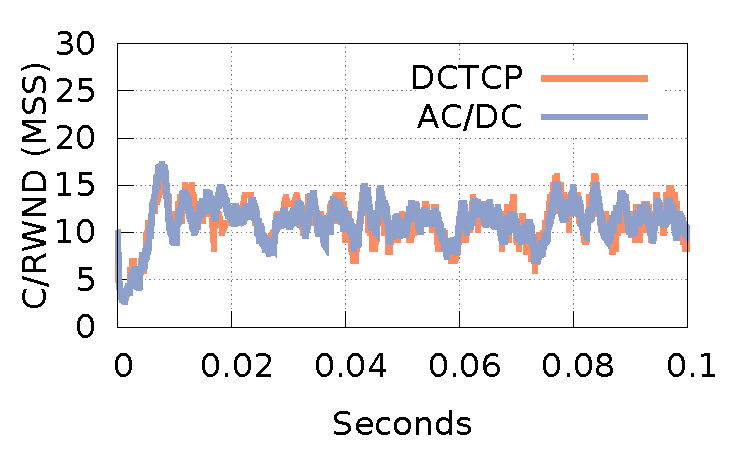
\includegraphics[width=\textwidth]{acdctcp/figures/cwnd_rwnd/newpara_refine/mtu1500_5flows_1/measure_cwnd_rwnd_gap_15k_5flows_0sec_100msec.pdf}
                \caption{First 100 ms of a flow.}
                \label{cwnd_rwnd_1500}
        \end{subfigure}
        \begin{subfigure}[b]{0.45\textwidth}
                \centering
                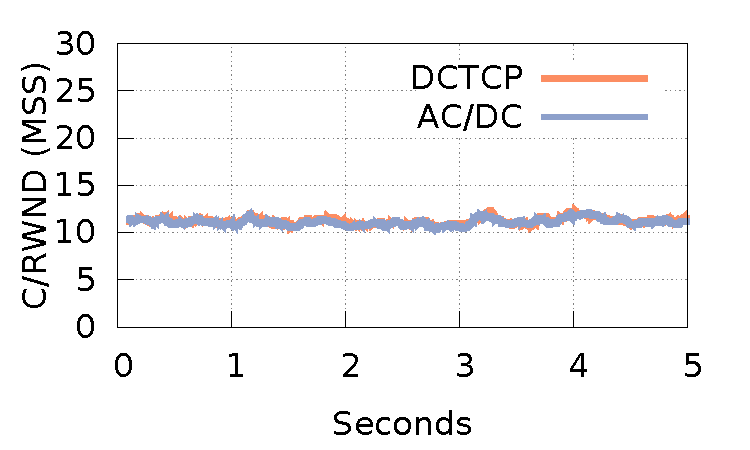
\includegraphics[width=\textwidth]{acdctcp/figures/cwnd_rwnd/moving-ave/measure_cwnd_rwnd_gap_15k_5flows_ave100.pdf}
                \caption{Moving average.}
                \label{cwnd_rwnd_1500_ave}
        \end{subfigure}

        \caption{~\acdc{}'s \rwnd{} tracks DCTCP's~\cwnd{} (1.5KB MTU).}
        \label{compare_cwnd_rwnd}
\end{figure}



%%who limits TCP throughput, CWND or RWND? CUBIC
\begin{figure}[!t]
        \centering
        \begin{subfigure}[b]{0.45\textwidth}
                \centering
                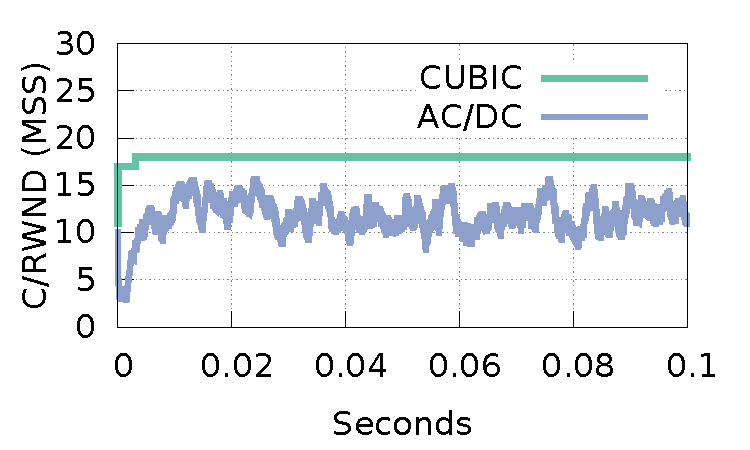
\includegraphics[width=\textwidth]{acdctcp/figures/cwnd_rwnd2/mtu1500_cubic/cubic_measure_cwnd_rwnd_gap_15k_5flows_0sec_100msec.pdf}
                \caption{Starting from 0 sec.}
                \label{who_limits_cwnd_rwnd_1500_0sec}
        \end{subfigure}
        \begin{subfigure}[b]{0.45\textwidth}
                \centering
                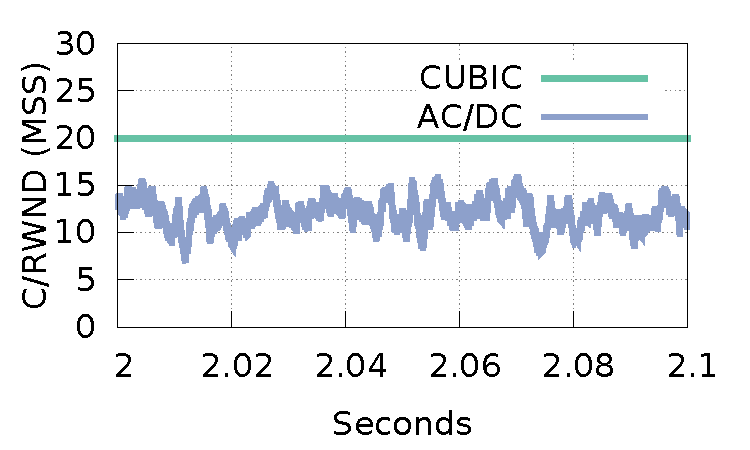
\includegraphics[width=\textwidth]{acdctcp/figures/cwnd_rwnd2/mtu1500_cubic/cubic_measure_cwnd_rwnd_gap_15k_5flows_2sec_100msec.pdf}
                \caption{Starting from 2 sec.}
                \label{who_limits_cwnd_rwnd_1500_2sec}
        \end{subfigure}
%        \begin{subfigure}[b]{0.225\textwidth}
%                \centering
%                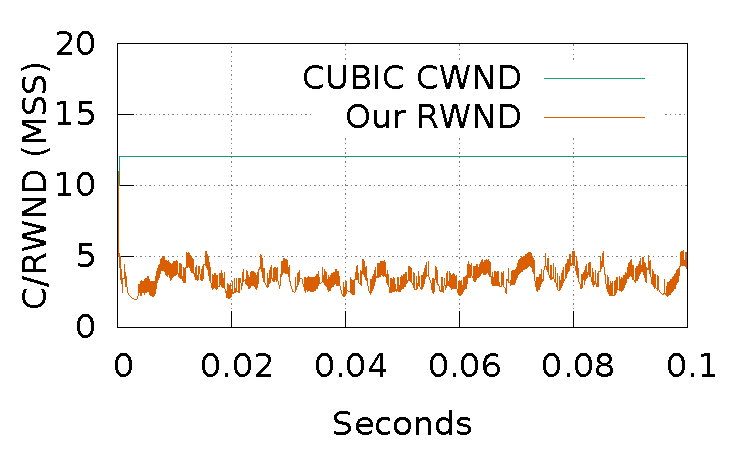
\includegraphics[width=\textwidth]{acdctcp/figures/cwnd_rwnd2/mtu9000_cubic/cubic_measure_cwnd_rwnd_gap_9k_5flows_0sec_100msec.pdf}
%                \caption{MTU9000: first 100 msec starting from second 0.}
%                \label{who_limits_cwnd_rwnd_9000_0sec}
%        \end{subfigure}
%        \begin{subfigure}[b]{0.225\textwidth}
%                \centering
%                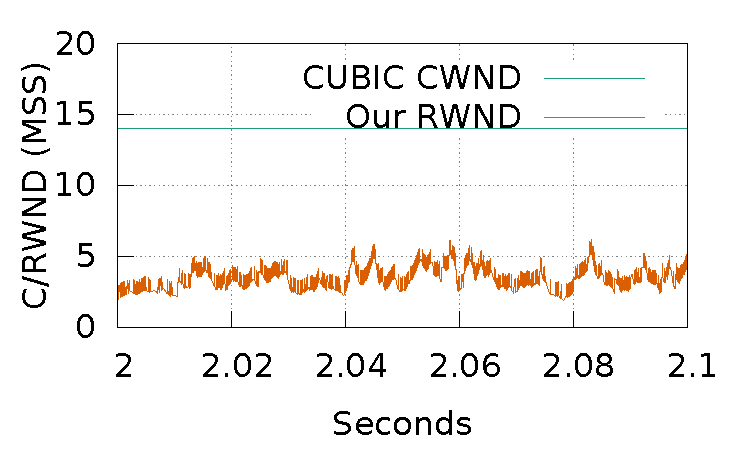
\includegraphics[width=\textwidth]{acdctcp/figures/cwnd_rwnd2/mtu9000_cubic/cubic_measure_cwnd_rwnd_gap_9k_5flows_2sec_100msec.pdf}
%                \caption{MTU9000: first 100 msec starting from second 2.}
%                \label{who_limits_cwnd_rwnd_9000_2sec}
%        \end{subfigure}
        \caption{Who limits TCP throughput when~\acdc{} is run with CUBIC? (1.5 KB MTU)}
        \label{who_limits_compare_cwnd_rwnd}
\end{figure}

\begin{figure}[!t]
        \centering
  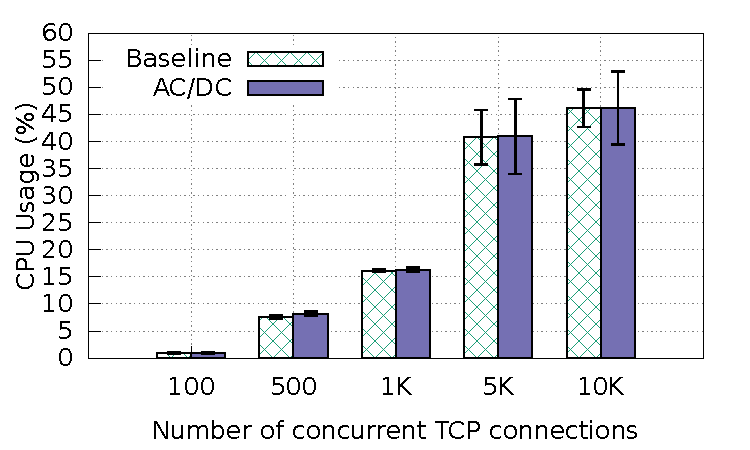
\includegraphics[width=0.5\textwidth]{acdctcp/figures/overhead/sender_15k_compare_cpu_witherrbar.pdf}
        \caption{CPU overhead: sender side (1.5KB MTU).}
        \label{cpu_overhead_sender_15k}
\end{figure}

\begin{figure}[!t]
        \centering
  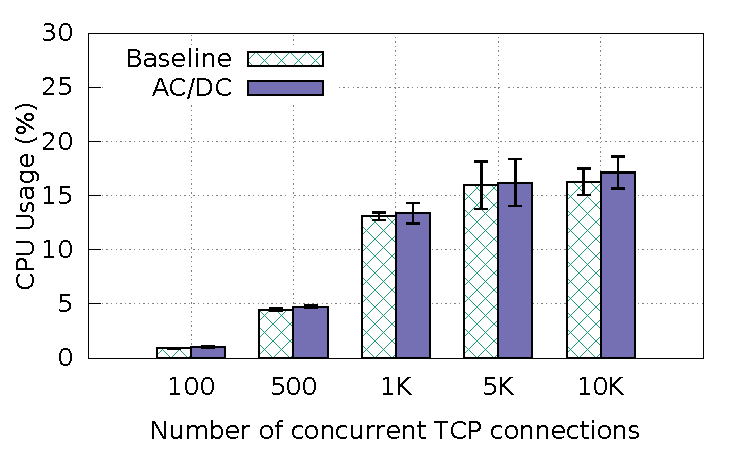
\includegraphics[width=0.5\textwidth]{acdctcp/figures/overhead/receiver_15k_compare_cpu_witherrbar.pdf}
        \caption{CPU overhead: receiver side (1.5KB MTU).}
        \label{cpu_overhead_receiver_15k}
\end{figure}


\begin{figure}[!t]
        \centering
  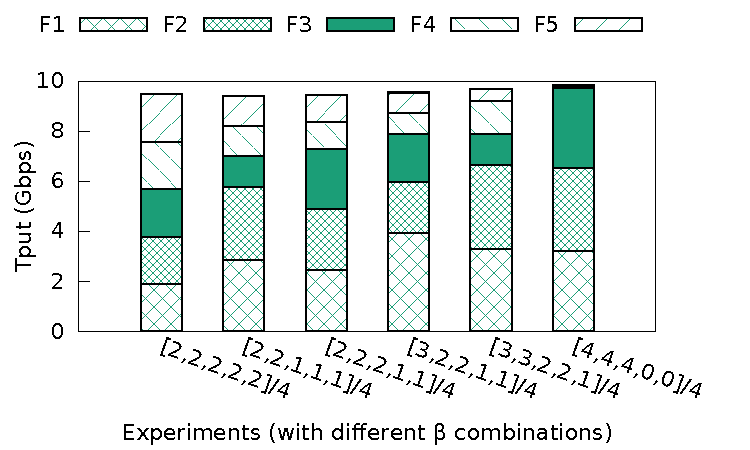
\includegraphics[width=0.5\textwidth]{acdctcp/figures/qos/qos_stacked.pdf}
        \caption{\crs{\acdc{} provides differentiated throughput via QoS-based CC. $\beta$ values are defined on a 4-point scale.}}
        \label{cc-qos}
\end{figure}

\tightparagraph{Tracking window sizes}
Next, we aim to understand how accurately~\acdc{} tracks DCTCP's performance at a finer level. The host's TCP
stack is set to DCTCP and our scheme runs in the vSwitch.
We repeat the experiment in Figure~\ref{dumbbell_topology} and measure the~\rwnd{} calculated by~\acdc{}. Instead
of over-writing the~\rwnd{} value in the ACKs, we simply log the value to a file. Thus, congestion is enforced by DCTCP
and we can capture DCTCP's~\cwnd{} by using {\tt tcpprobe}~\cite{tcp-probe}. We align the~\rwnd{} and~\cwnd{} values by timestamps and sequence
numbers and show a timeseries in Figure~\ref{compare_cwnd_rwnd}. Figure~\ref{cwnd_rwnd_1500} shows both windows for the
first 100 ms of a flow and shows that~\acdc{}'s calculated window closely tracks DCTCP's. Figure~\ref{cwnd_rwnd_1500_ave} 
shows the windows over a 100ms moving average are also similar. This suggests it is possible to accurately recreate congestion
control in the vSwitch.~\crs{These results are obtained with 1.5KB MTU. Trends for 9KB MTU are similar but the window sizes are smaller}.

We were also interested to see how often~\acdc{}'s congestion window takes effect. We rerun the experiment~\crs{(MTU is still 1.5KB)}, but set
the host TCP stack to CUBIC. The~\rwnd{} computed by~\acdc{} is both written into the ACK and logged to a file. We again
use {\tt tcpprobe} to measure CUBIC's~\cwnd{}. Figure~\ref{who_limits_compare_cwnd_rwnd} is a timeseries (one graph from the
start of the experiment and one graph 2 seconds in) that shows~\acdc{}'s
congestion control algorithm is indeed the limiting factor.
In the absence of loss or ECN markings, traditional TCP stacks do not severely reduce~\cwnd{} and thus
\acdc{}'s~\rwnd{} becomes the main enforcer of a flow's congestion control. Because DCTCP 
is effective at reducing loss and~\acdc{} hides ECN feedback from the host TCP stack,
~\acdc{}'s enforcement is applied often.
%As before, 9KB MTU results showed similar trends.

%
%\begin{figure}[!htb]
%        \centering
%  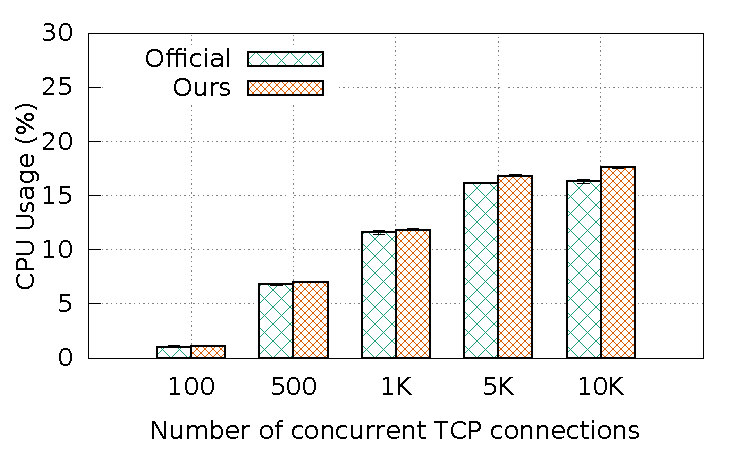
\includegraphics[width=0.45\textwidth]{acdctcp/figures/overhead/sender_9k_compare_cpu_witherrbar.pdf}
%        \caption{CPU overhead: sender side (9K MTU). The 10G NIC is saturated when there are more than 1K TCP connections.
%		CPU usage refers to the CPU usage of the whole server (12 Intel(R) Xeon(R) CPU E5649@2.53GHz processors)
%                measured by ``sar (sysstat)''.}
%        \label{cpu_overhead_sender_9k}
%\end{figure}
%
%\begin{figure}[!htb]
%        \centering
%  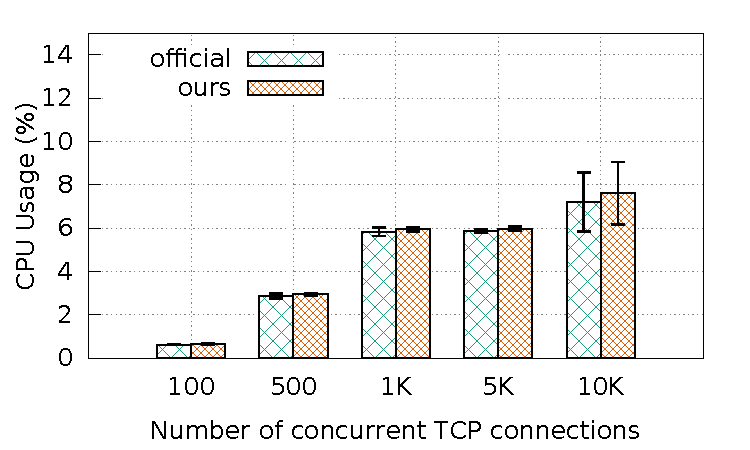
\includegraphics[width=0.45\textwidth]{acdctcp/figures/overhead/receiver_9k_compare_cpu_witherrbar.pdf}
%        \caption{CPU overhead: receiver side (9K MTU). The 10G NIC is saturated when there are more than 1K TCP connections.
%		CPU usage refers to the CPU usage of the whole server (12 Intel(R) Xeon(R) CPU E5649@2.53GHz processors)
%                measured by ``sar (sysstat)''}
%        \label{cpu_overhead_receiver_9k}
%\end{figure}
%

\tightparagraph{CPU overhead}
We measure the CPU overhead of~\acdc{} by connecting two servers to a single switch. 
Multiple simultaneous TCP flows are started from one server to the other and the total CPU utilization
is measured on the sender and receiver using {\tt sar}. Each flow is given time to perform the TCP handshake
and when all are connected, each TCP client sends with a demand of 10 Mbps by sending 128KB bursts every 100 milliseconds (so 1,000 connections saturate the 10 Gbps link). 
The~\crs{system-wide} CPU overhead of~\acdc{} compared to the~\crs{system-wide} CPU overhead of baseline (\ie{}, just OVS) 
is shown for the sender in Figure~\ref{cpu_overhead_sender_15k}
 and the receiver in Figure~\ref{cpu_overhead_receiver_15k}.~\crs{Error bars show standard deviation over 50 runs.
While~\acdc{} increases CPU usage in all cases, the increase is negligible. The largest difference is less than one percentage point: 
the baseline and~\acdc{} have 16.27\% and 17.12\% utilization, respectively for 10K flows at the receiver.
%Even when scaling to 
%10,000 connections, the CPU overhead of our scheme is less than 1\%.
The results are shown with 1.5KB MTU because smaller packets incur higher overhead. Note experiments with 9KB MTU have similar trends.}
%https://en.wikipedia.org/wiki/Relative_change_and_difference
%https://www.mathsisfun.com/percentage-points.html


%%% other TCP variants %%%
\begin{table*}[!t]
\tiny
\begin{center}
\begin{tabular}{ |c|c|c|c|c|c|c|c|c| }
 \hline
 \multirow{2}{*}{CC Variants} & \multicolumn{2}{|c|}{50$^{th}$ percentile RTT ($\mu$s)} & \multicolumn{2}{|c|}{99$^{th}$ percentile RTT ($\mu$s)} & \multicolumn{2}{|c|}{Avg Tput (Gbps)} & \multicolumn{2}{|c|}{Fairness Index}\\
 \cline{2-9}
       &  mtu=1.5KB & mtu=9KB & mtu=1.5KB & mtu=9KB & mtu=1.5KB & mtu=9KB & mtu=1.5KB & mtu=9KB\\
 \hline
 \hline
 CUBIC* &  3232     &   3448    &   3641     &  3865     &   1.89    & 1.98   &  0.85   &   0.98\\
 DCTCP* &  128      &   142    &   232    &   259    &   1.89    &   1.98  &  0.99    &   0.99\\
 \hline
 \hline
 CUBIC &   128     &   142    &    231    &   252    &   1.89    &  1.98   &  0.99    &  0.99 \\
 Reno  &   120     &   149    &    235    &   248    &   1.89    &  1.97   &  0.99    &  0.99 \\
DCTCP  &   129     &   149    &    232    &   266    &   1.88    &  1.98   &  0.99    &  0.99 \\
Illinois  &   134     &   152    &    215    &  262     &   1.89    &  1.97   &  0.99    &  0.99 \\
HighSpeed  &   119     &  147     &    224    &  252     &   1.88    & 1.97    &  0.99    & 0.99  \\
 Vegas  &   126     &   143    &    216    &    251   &   1.89    &  1.97   &  0.99    &  0.99 \\

 \hline

\end{tabular}
\caption{\acdc{} works with many congestion control variants.~\crs{Legend:}
        CUBIC*: CUBIC + standard OVS, switch WRED/ECN marking off.
        DCTCP*: DCTCP + standard OVS, switch WRED/ECN marking on.
        Others: different CCs + \acdc{}, switch WRED/ECN marking on.}
\label{other_cc_variants}
\end{center}
\end{table*}

%%%convergence %%%
\begin{figure*}[!t]
        \centering
        \begin{subfigure}[b]{0.3\textwidth}
                \centering
                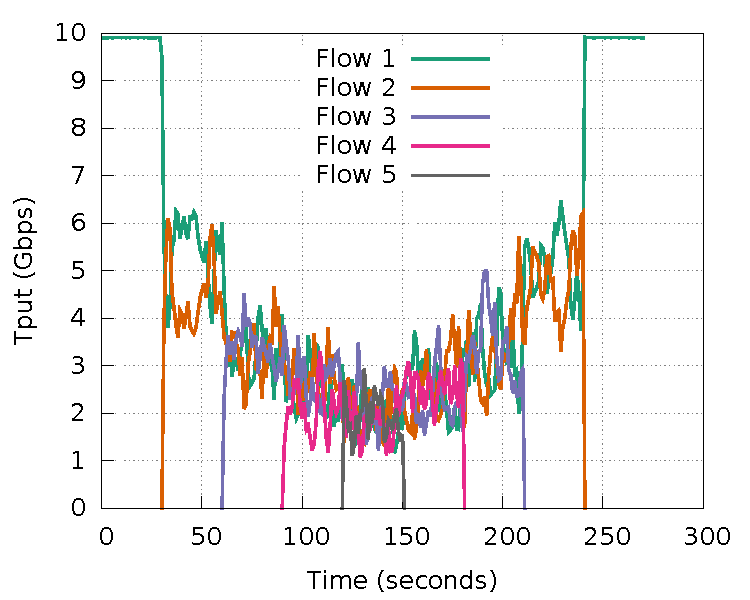
\includegraphics[width=\textwidth]{acdctcp/figures/convergence/flowcontrolOFF/tcp_flowcontrolOFF_convergence.pdf}
                \caption{CUBIC convergence test.}
                \label{cubic_convergence}
        \end{subfigure}
        \begin{subfigure}[b]{0.3\textwidth}
                \centering
                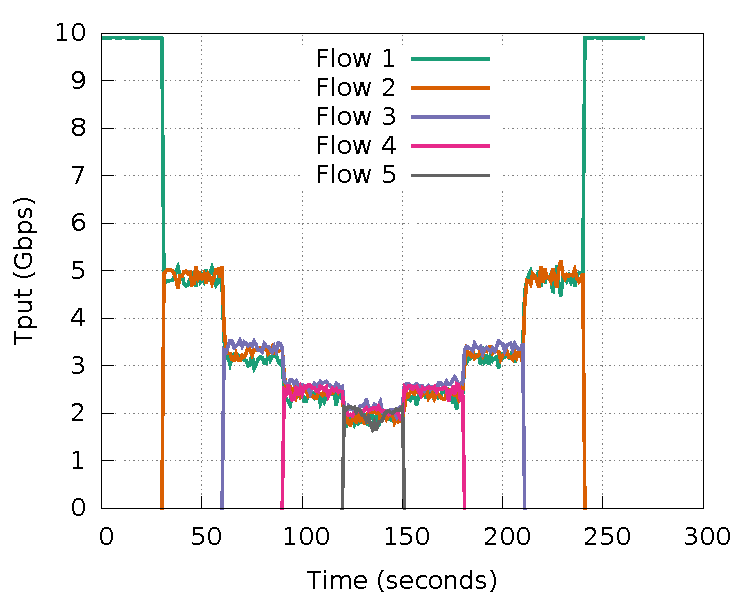
\includegraphics[width=\textwidth]{acdctcp/figures/convergence/flowcontrolOFF/dctcp_flowcontrolOFF_convergence.pdf}
                \caption{DCTCP convergence test.}
                \label{dctcp_convergence}
        \end{subfigure}
        \begin{subfigure}[b]{0.3\textwidth}
                \centering
                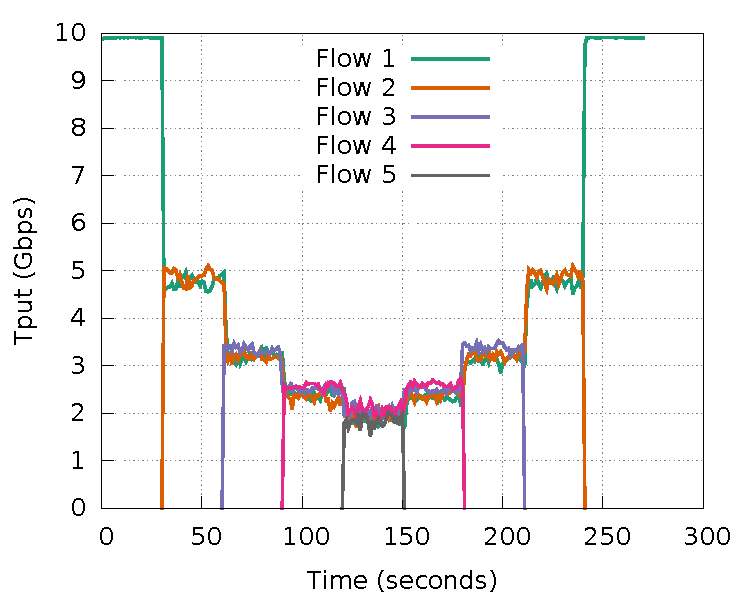
\includegraphics[width=\textwidth]{acdctcp/figures/convergence/flowcontrolOFF/ovsdctcp_flowcontrolOFF_convergence.pdf}
                \caption{\acdc{} convergence test.}
                \label{ovsdctcp_convergence}
        \end{subfigure}
        \caption{~\crs{Convergence tests: flows are added, then removed, every 30 secs.~\acdc{} performance matches DCTCP.}}
        \label{convergence_test}
\end{figure*}


\tightparagraph{~\acdc{} flexibility}~\acdc{} aims to provide a degree of control and flexibility over tenant TCP stacks. 
We consider two cases.
First,~\acdc{} should work effectively, regardless of the tenant TCP stack.
Table~\ref{other_cc_variants} shows the performance of our scheme when various TCP congestion control algorithms
are configured on the host. Data is collected over 10 runs lasting 20 seconds each on the dumbbell topology (Figure~\ref{dumbbell_topology}). 
The first two rows of the table, CUBIC* and DCTCP*, show the performance of each stack with an 
unmodified OVS. The next six rows show the performance of a given host stack with~\acdc{} running DCTCP in OVS.
The table shows~\acdc{} can effectively track the performance of DCTCP*, meaning 
it is compatible with popular delay-based (Vegas) and loss-based (Reno, CUBIC, etc) stacks.

Second,~\acdc{} enables an administrator to assign different 
congestion control algorithms on a per-flow basis. 
%For example, congestion control algorithms shown to optimize WAN performance, 
%such as Compound TCP~\cite{tan2006compound}, can be employed on front-end
%web server traffic, while DCTCP can be used for intra-DC back-end traffic.
For example,~\acdc{} can provide the flexibility to implement QoS through differentiated congestion control. 
We fix the host TCP stack to CUBIC and alter~\acdc{}'s congestion control for each flow
by setting the $\beta$ value (in Equation~\ref{eqn:cc-qos}) for each flow in the dumbbell topology. 
Figure~\ref{cc-qos} shows the throughput achieved by each flow, 
along with its $\beta$ setting.~\acdc{} is 
able to provide relative bandwidth allocation to each flow based on $\beta$. 
Flows with the same $\beta$ value get similar throughputs and flows with higher $\beta$ values 
obtain higher throughput.
The latencies (not shown) remain consistent with
previous results.


%%%coexistence %%%
\begin{figure}[!t]
        \centering
        \begin{subfigure}[b]{0.45\textwidth}
                \centering
                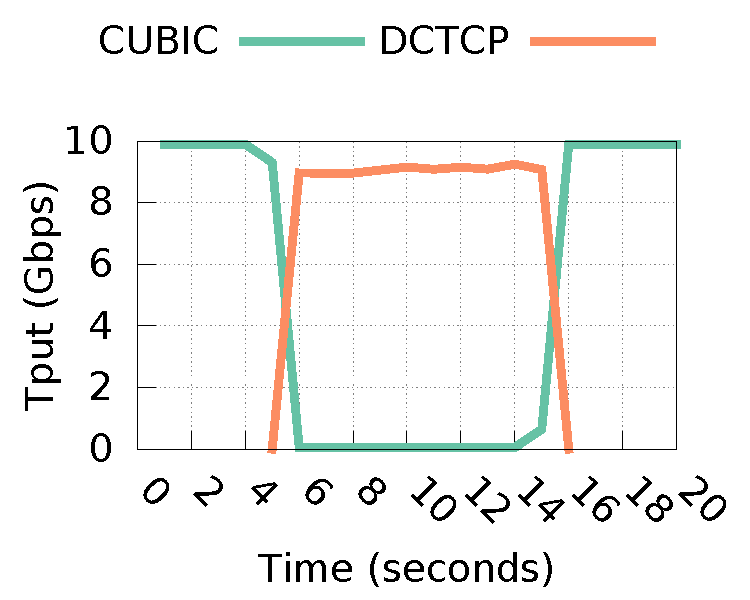
\includegraphics[width=\textwidth]{acdctcp/figures/micro2flows/coexitence/cubic_dctcp_coexistence_official.pdf}
                \caption{Default.}
                \label{coexistence_tput_ovs}
        \end{subfigure}
        \begin{subfigure}[b]{0.45\textwidth}
                \centering
                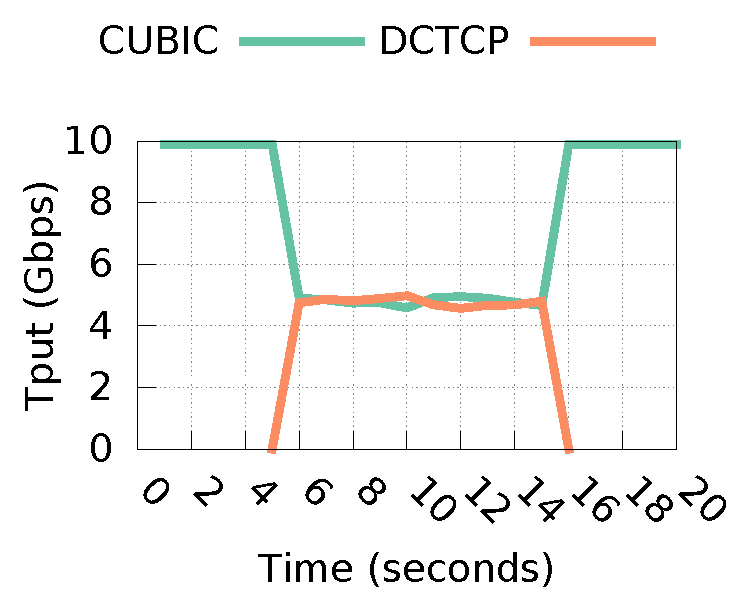
\includegraphics[width=\textwidth]{acdctcp/figures/micro2flows/coexitence/cubic_dctcp_coexistence_acdctcp.pdf}
                \caption{\acdc{}.}
                \label{coexistence_tput_ovsdctcp}
        \end{subfigure}
        \caption{(a) CUBIC gets little throughput when competing with DCTCP.
		 (b) With \acdc{}, CUBIC and DCTCP flows get fair share.}
        \label{coexistence_tput}
\end{figure}

\begin{figure}[!t]
        \centering
  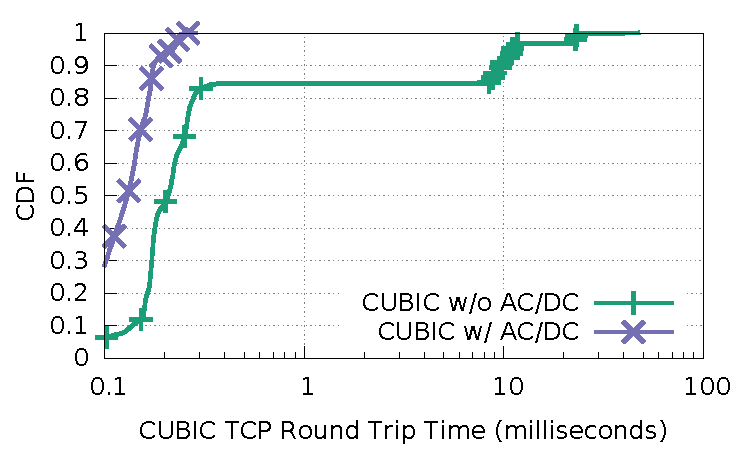
\includegraphics[width=0.5\textwidth]{acdctcp/figures/micro2flows/coexitence/sockperf_and_droprate/coexistence_sockperf.pdf}
        \caption{CUBIC experiences high RTT when competing with DCTCP.~\acdc{} fixes this issue.}
        \label{coexistence_sockperf_droprate}
\end{figure}

\begin{figure}[!t]
        \centering
%        \begin{subfigure}[b]{0.24\textwidth}
%                \centering
%                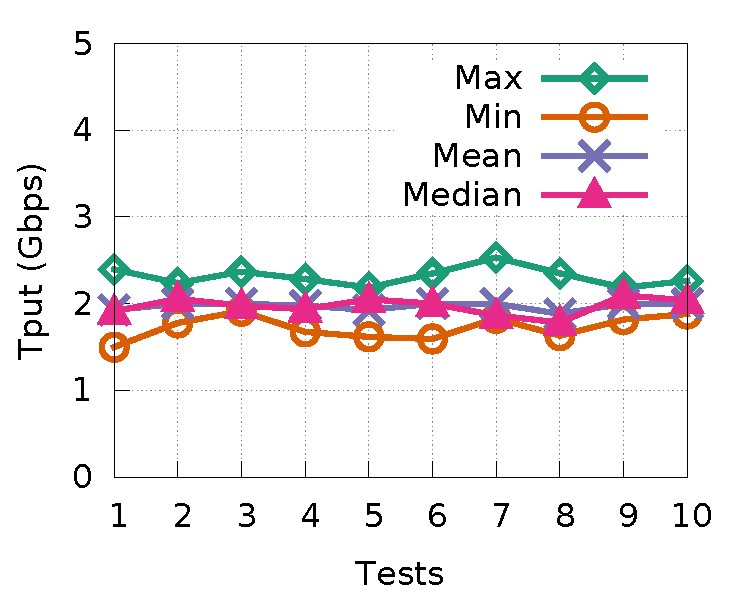
\includegraphics[width=\textwidth]{acdctcp/figures/tput_fairness/default_all_cubic_tput.pdf}
%                \caption{All CUBIC.}
%                \label{fairness_all_cubic}
%        \end{subfigure}
%        \begin{subfigure}[b]{0.24\textwidth}
%                \centering
%                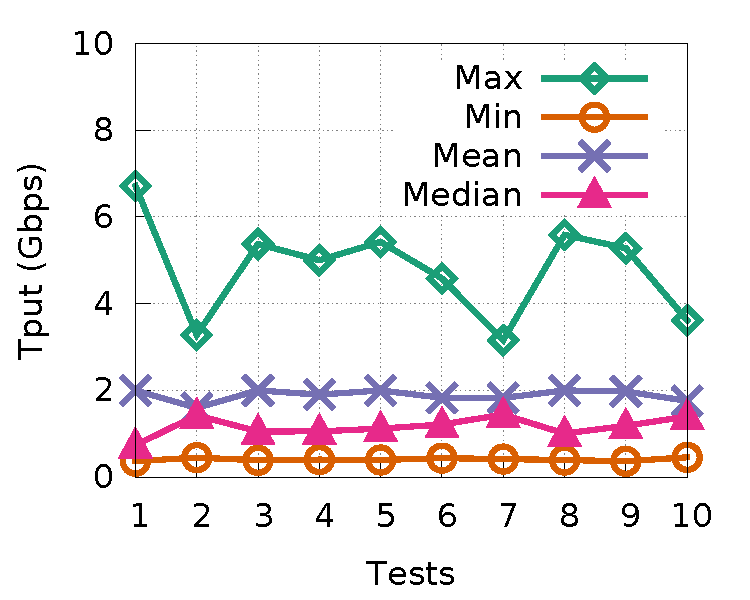
\includegraphics[width=\textwidth]{acdctcp/figures/tput_fairness/default_5CC_tput.pdf}
%                \caption{5 different CCs.}
%                \label{fairness_5CC}
%        \end{subfigure}
        \begin{subfigure}[b]{0.45\textwidth}
                \centering
                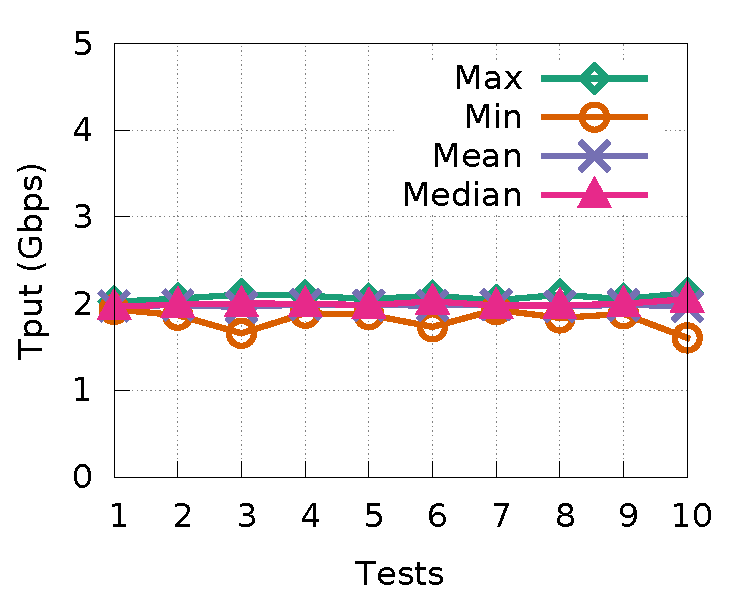
\includegraphics[width=\textwidth]{acdctcp/figures/tput_fairness/ecn_all_dctcp_tput.pdf}
                \caption{All DCTCP.}
                \label{fairness_5CC_with_dctcp}
        \end{subfigure}
        \begin{subfigure}[b]{0.45\textwidth}
                \centering
                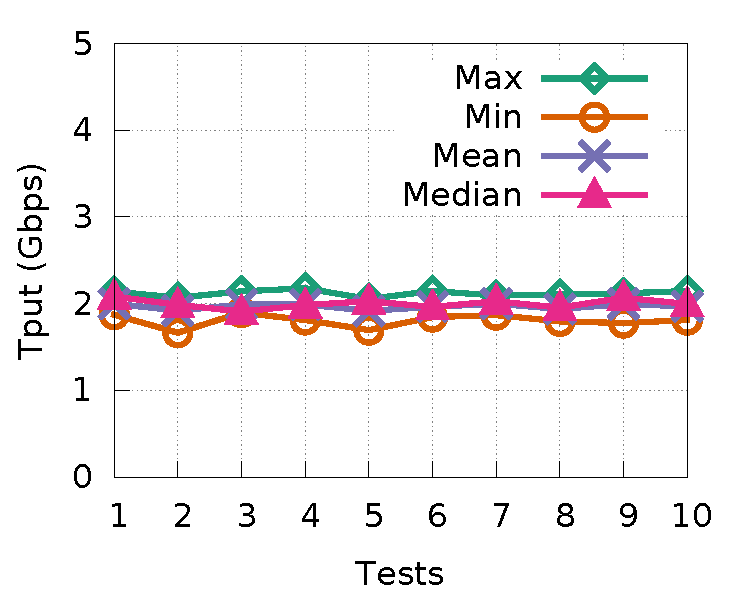
\includegraphics[width=\textwidth]{acdctcp/figures/tput_fairness/liquid_5CC_tput.pdf}
                \caption{5 different CCs (\acdc{}).}
                \label{fairness_5CC_with_ours}
        \end{subfigure}
	\caption{~\crs{\acdc{} improves fairness when VMs implement different CCs. DCTCP performance shown for reference.}} 
 	\label{tput_fairness_coexistence}
\end{figure}	


\tightparagraph{Fairness}
Three different experiments are used to demonstrate fairness. First, we show~\acdc{} can mimic DCTCP's 
behavior in converging to fair throughputs. We repeat the experiment originally performed 
by Alizadeh~\cite{alizadeh2011data} and Judd~\cite{judd2015nsdi} by 
adding a new flow every 30 seconds on a bottleneck link and then reversing the process. 
The result is shown in Figure~\ref{convergence_test}.
Figure~\ref{cubic_convergence} shows CUBIC's problems converging to fair allocations.
Figures~\ref{dctcp_convergence}
and~\ref{ovsdctcp_convergence} show DCTCP and~\acdc{} performance, respectively.~\acdc{} tracks DCTCP's behavior.
CUBIC's drop rate is 0.17\% while DCTCP's and \acdc{}'s is 0\%. 
%Note that as mentioned in~\cite{judd2015nsdi}, CUBIC's 
%performance can be improved by manually altering the socket buffer size, 
%but let applications sizing it in practice is hard. DCTCP, and thus
%our scheme, do not need this optimization, 
%thus demonstrating one additional benefit of our approach.

The second experiment is also repeated from Judd's paper~\cite{judd2015nsdi}. 
ECN-capable and non-ECN-capable flows do not coexist well because switches
drop non-ECN packets when the queue length is larger than the marking threshold. Figure~\ref{coexistence_tput_ovs}
shows the throughput of CUBIC suffers when CUBIC (with no ECN) and DCTCP (with ECN) traverse the same bottleneck link.
Figure~\ref{coexistence_tput_ovsdctcp} shows~\acdc{} alleviates this problem 
because it forces all flows to become ECN-capable.
Figure~\ref{coexistence_sockperf_droprate} shows CUBIC's RTT is extremely high
in the first case because switches drop non-ECN packets (the loss rate is 0.18\%) and thus
there is a significant number of retransmissions. However,~\acdc{} eliminates 
this issue and reduces latency.
%\emph{\acdc{} makes low latency possible in production data center networks where
%incremental deployment is the norm and transport diversity must be supported}.

The last experiment examines the impact of having multiple TCP stacks on the same fabric. 
Five flows with different congestion control algorithms (CUBIC, Illinois, HighSpeed, New Reno and Vegas) are started
on the dumbbell topology. This is the same experiment as in Figure~\ref{tput_unfair}.
Figure~\ref{fairness_5CC_with_dctcp} shows what happens if all
flows are configured to use DCTCP and Figure~\ref{fairness_5CC_with_ours} shows when
the five different stacks traverse~\acdc{}. We can see~\acdc{} closely tracks the ideal case of
all flows using DCTCP, and~\acdc{} and DCTCP provide better fairness than all CUBIC (Figure~\ref{unfairness_all_cubic}).
%The median and 99.9\% TCP RTTs for all CUBIC, 5 different CCs, 5 different CCs with
%our logic and all DCTCP are: 3.5 ms, 3.9 ms; 3.4 ms, 4.0 ms; 146 $\mu$s, 306 $\mu$s;
%147 $\mu$s, 317 $\mu$s. Both~\acdc{} and DCTCP obtain a Jain's fairness index greater than 0.99.


\iffalse
\tightparagraph{Different MTU sizes}
We set MTU size to 1500 bytes and run the tests on the dumbbell topology (Figure~\ref{dumbbell_topology})
with 5 flows competing for
a 10G bottleneck link. \acdc{} gets 1.87Gbps average flow throughput. DCTCP gets 1.88Gbps average flow throughput. 
Both have a Jain's fairness index greater than 0.99. TCP CUBIC gets 1.89 average flow throughput and a fairness index of 0.85.
The 50$^{th}$ and 99.9$^{th}$ percentile TCP RTT for \acdc{} (DCTCP, CUBIC) are 139$\mu$s (136$\mu$s, 3.2ms) and
359$\mu$s (342$\mu$s, 3.7ms), respectively.
~\eric{KEQIANG: please look at this paragraph and see how it fits in the
"Canonical Topologies" paragraph. Our numbers should be consistent. We can 
remove this paragraph afterwards.}
\fi

\subsection{Macrobenchmarks}
\label{macro}

%%%%%%%%%%using figures to present incast: tput, fariness, droprate, TCP RTT
\begin{figure}[!t]
        \centering
        \begin{subfigure}[b]{0.45\textwidth}
                \centering
                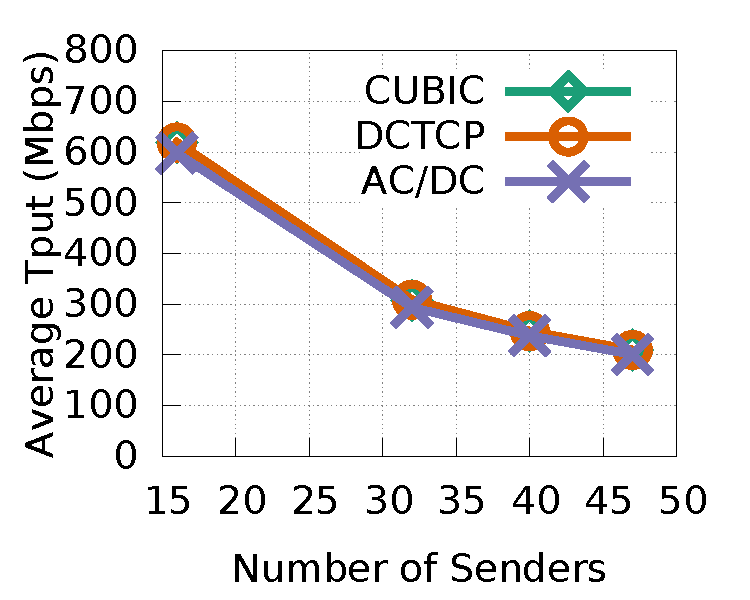
\includegraphics[width=\textwidth]{acdctcp/figures/incast/plots9k/incast_tput_vary_sender.pdf}
                \caption{Average throughput.}
                \label{incast_9k_tput}
        \end{subfigure}
        \begin{subfigure}[b]{0.45\textwidth}
                \centering
                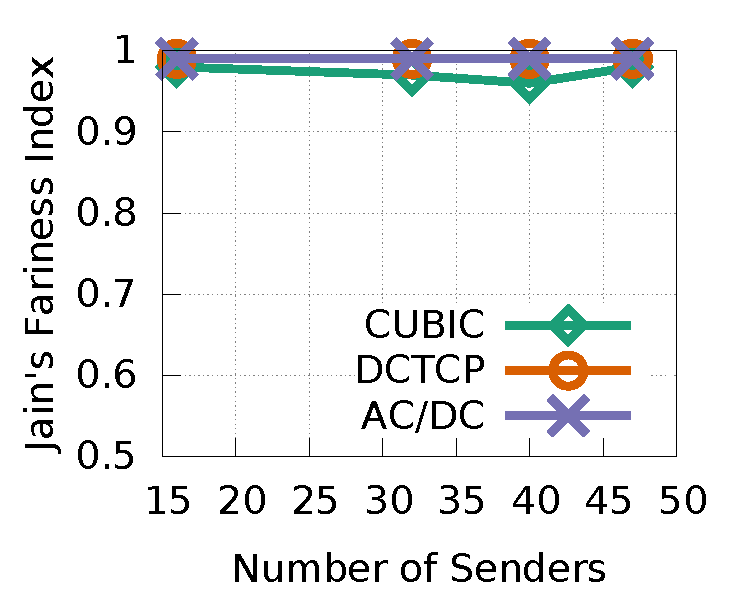
\includegraphics[width=\textwidth]{acdctcp/figures/incast/plots9k/incast_fairness_vary_sender.pdf}
                \caption{Fairness.}
                \label{incast_9k_fariness}
        \end{subfigure}
        \caption{Many to one incast: throughput and fairness.}
        \label{incast_9k_tput_fairness}
\end{figure}

\begin{figure*}[!t]
        \centering
        \begin{subfigure}[b]{0.3\textwidth}
                \centering
                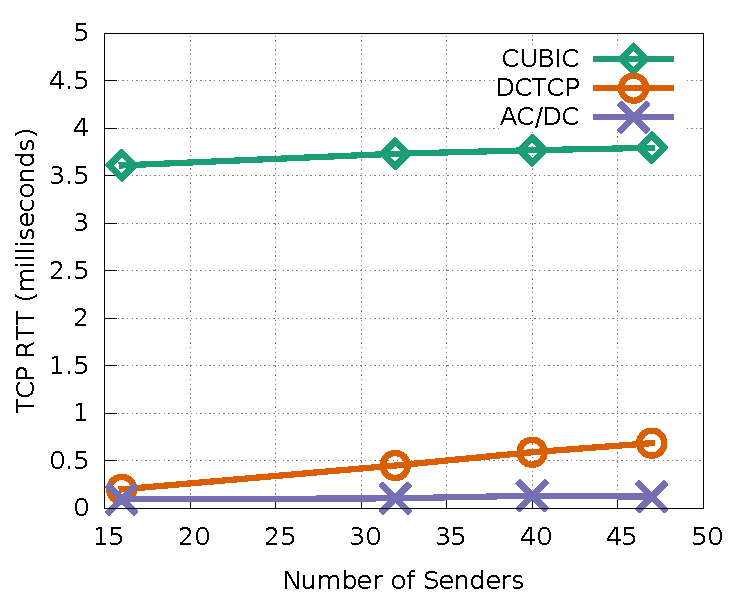
\includegraphics[width=\textwidth]{acdctcp/figures/incast/plots9k/incast_sockperf50th_vary_sender.pdf}
                \caption{50$^{th}$ percentile RTT.}
                \label{incast_9k_50th_sockperf}
        \end{subfigure}
        \begin{subfigure}[b]{0.3\textwidth}
                \centering
                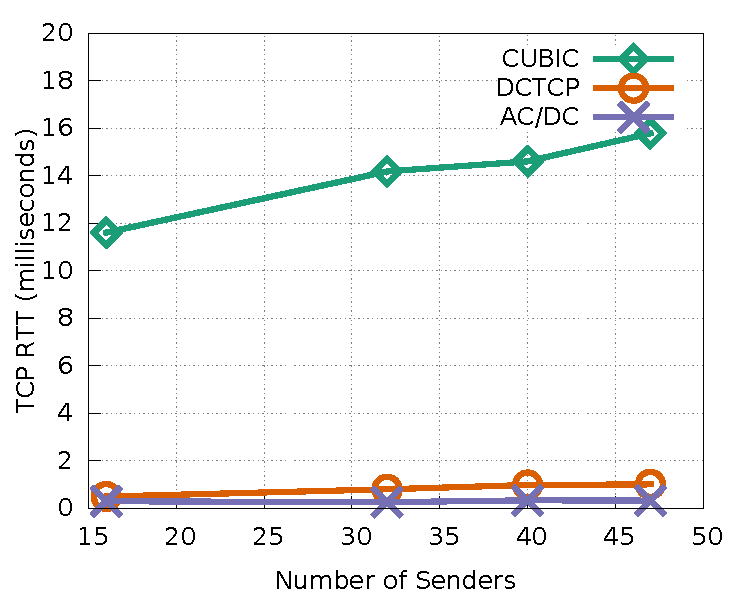
\includegraphics[width=\textwidth]{acdctcp/figures/incast/plots9k/incast_sockperf999th_vary_sender.pdf}
                \caption{99.9$^{th}$ percentile RTT.}
                \label{incast_9k_999th_sockperf}
        \end{subfigure}
        \begin{subfigure}[b]{0.3\textwidth}
                \centering
                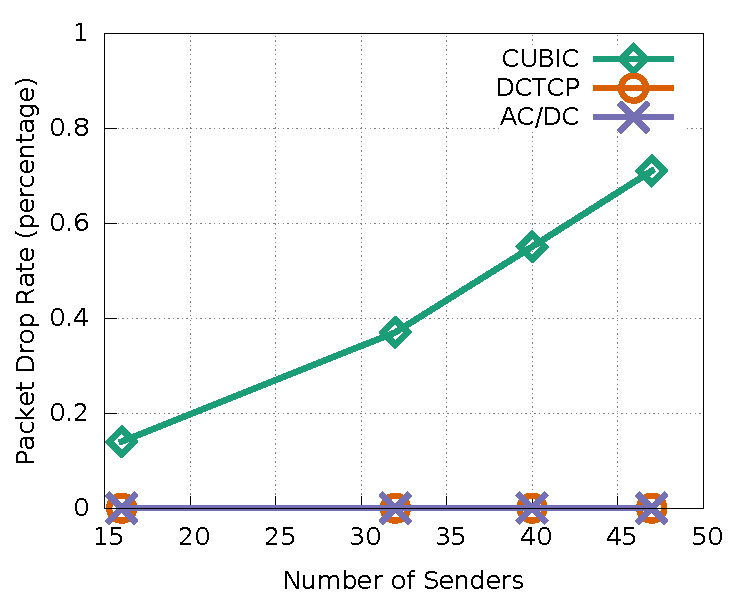
\includegraphics[width=\textwidth]{acdctcp/figures/incast/plots9k/incast_droprate_vary_sender.pdf}
                \caption{Packet drop rate.}
                \label{incast_9k_droprate}
        \end{subfigure}
        \caption{Many to one incast: RTT and packet drop rate.\crs{~\acdc{} can reduce DCTCP's RTT by limiting window sizes.}}
        \label{incast_9k_sockperf_droprate}
\end{figure*}


\begin{figure}[!t]
        \centering
  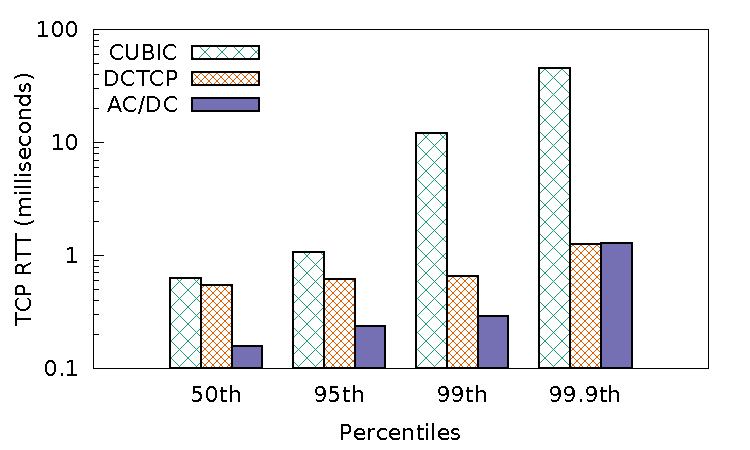
\includegraphics[width=0.5\textwidth]{acdctcp/figures/incast/pressure/incast_pressure_compare_sockperf.pdf}
        \caption{TCP RTT when almost all ports are congested.}
        \label{sockperf_pressure_incast}
\end{figure}

%
%

\iffalse
\begin{figure*}[!t]
        \centering
        \begin{subfigure}[b]{0.45\textwidth}
                \centering
                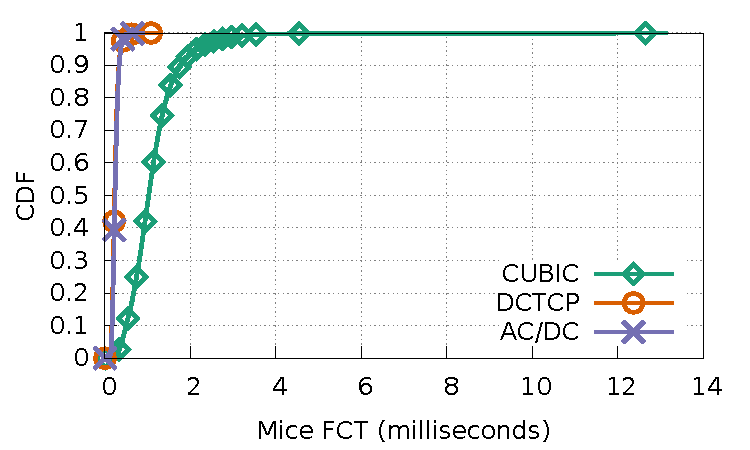
\includegraphics[width=\textwidth]{acdctcp/figures/macro_benchmarks/macro_4stride/stride4_mice16KB_fct.pdf}
                \caption{Mice flow completion times.}
                \label{macro_4stride_mice_fct}
        \end{subfigure}
        \begin{subfigure}[b]{0.45\textwidth}
                \centering
                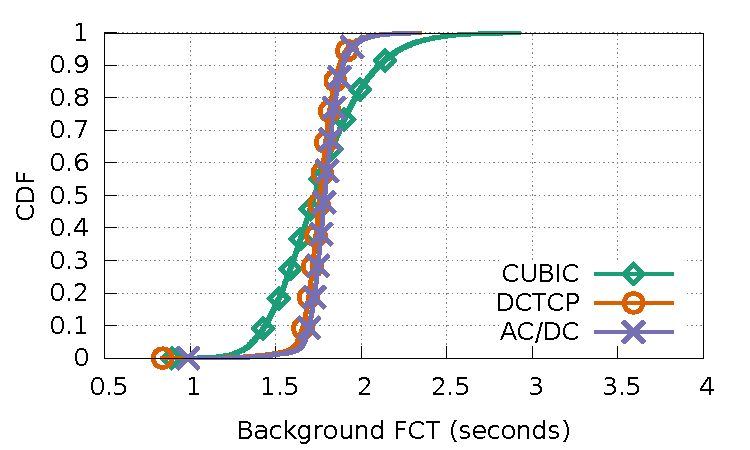
\includegraphics[width=\textwidth]{acdctcp/figures/macro_benchmarks/macro_4stride/stride4_big512MB_fct.pdf}
                \caption{Background flow completion times.}
                \label{macro_4stride_background_fct}
        \end{subfigure}
        \caption{CDF of mice and background FCTs in concurrent stride workload.}
        \label{macro_4stride_fct}
\end{figure*}

\begin{figure*}[!t]
        \centering
        \begin{subfigure}[b]{0.45\textwidth}
                \centering
                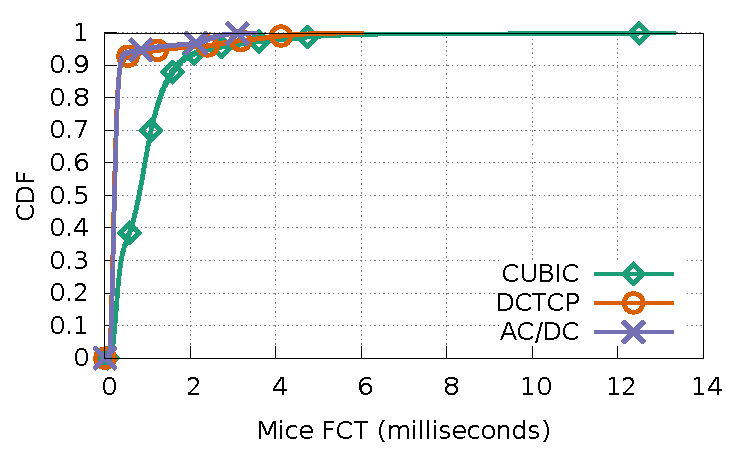
\includegraphics[width=\textwidth]{acdctcp/figures/macro_benchmarks/shuffle_17hosts/shuffle_mice16KB_fct.pdf}
                \caption{Mice flow completion times.}
                \label{macro_shuffle_mice_fct}
        \end{subfigure}
        \begin{subfigure}[b]{0.45\textwidth}
                \centering
                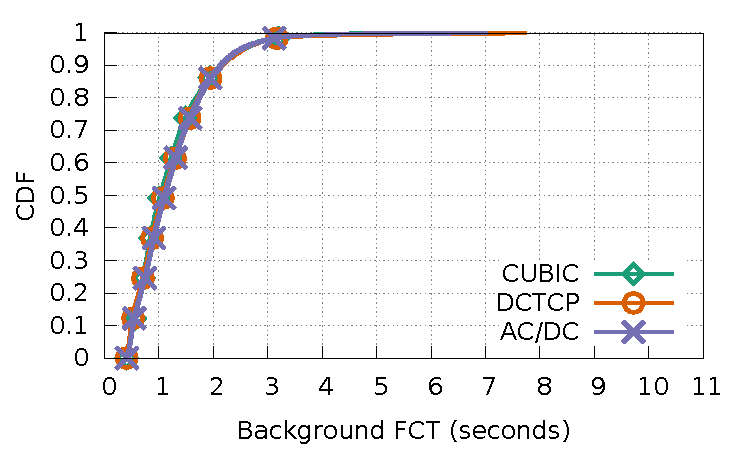
\includegraphics[width=\textwidth]{acdctcp/figures/macro_benchmarks/shuffle_17hosts/shuffle_big512MB_fct.pdf}
                \caption{Background flow completion times.}
                \label{macro_shuffle_background_fct}
        \end{subfigure}
        \caption{CDF of mice and background FCTs in shuffle workload.}
        \label{macro_shuffle_fct}
\end{figure*}

\begin{figure*}[!t]
        \centering
        \begin{subfigure}[b]{0.45\textwidth}
                \centering
                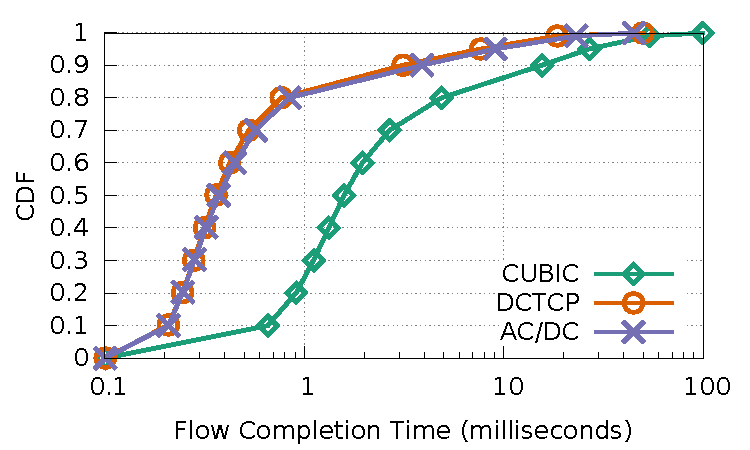
\includegraphics[width=\textwidth]{acdctcp/figures/macro_benchmarks/trace-driven/trace_driven_workload_dctcp_senders5_10points.pdf}
                \caption{Web-search workload.}
                \label{trace-driven-searching-fct}
        \end{subfigure}
        \begin{subfigure}[b]{0.45\textwidth}
                \centering
                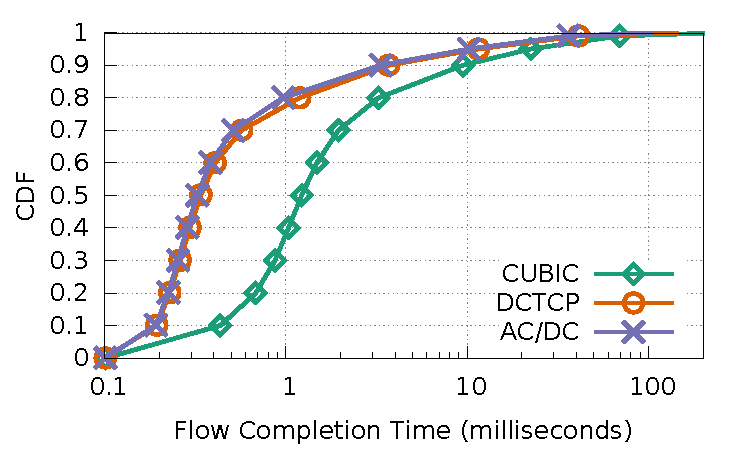
\includegraphics[width=\textwidth]{acdctcp/figures/macro_benchmarks/trace-driven/trace_driven_workload_conga_senders5_10points.pdf}
                \caption{Data-mining workload.}
                \label{trace-driven-data-mining-fct}
        \end{subfigure}
        \caption{CDF of mice ($<$10KB) FCT in web-search and data-mining workloads.}
        \label{macro-trace-driven-fct}
\end{figure*}
\fi


In this section we attach all servers to a single switch and
run a variety of workloads to better understand
how well~\acdc{} tracks DCTCP's performance. Experiments are run for 10 minutes. A simple TCP application
sends messages of specified sizes to measure FCTs.

\tightparagraph{Incast}
In this section, we evaluate incast scenarios.
To scale the experiment, 17 physical servers are equipped with four NICs each
and one flow is allocated per NIC.
In this way, incast can support up to 47-to-1 fan-in (our switch only has 48 ports).
We measure the extent of incast by increasing the number of concurrent senders to 16, 32, 40 and 47.
Figure~\ref{incast_9k_tput_fairness} shows throughput and fairness results.
Both DCTCP and \acdc{} obtain a fairness index greater than 0.99 and get comparable throughput as CUBIC.
Figure~\ref{incast_9k_sockperf_droprate} shows the RTT and packet drop rate results.
When there are 47 concurrent senders, DCTCP can reduce median RTT by 82\% and \acdc{} can reduce by 97\%;
DCTCP can reduce 99.9$^{th}$ percentile RTT by 94\% and \acdc{} can reduce by 98\%.
Both DCTCP and \acdc{} have 0\% packet drop rate. It is curious that~\acdc{}’s
performance is better than DCTCP when the number of senders increases (Figure~\ref{incast_9k_50th_sockperf}).
The Linux DCTCP code puts a lower bound of 2 packets on \cwnd{}.
In incast, we have up to 47 concurrent competing flows and
the network's MTU size is 9KB. In this case, the lower bound is too high,
so DCTCP's RTT increases gradually with the number of senders.
This issue was also found in~\cite{judd2015nsdi}.~\acdc{} controls \rwnd{} (which is in bytes)
instead of \cwnd{} (which is in packets) and \rwnd{}'s lowest value can be much smaller than 2*MSS.
We verified modifying~\acdc{}'s lower bound caused identical behavior.

\crs{The second test aims to put pressure on the switch's dynamic
buffer allocation scheme, similar to an experiment in the DCTCP paper~\cite{alizadeh2011data}.}
To this end, we aim to congest every switch port.
The 48 NICs are split into 2 groups: group $A$ and $B$.
Group $A$ has 46 NICs and $B$ has 2 (denoted $B_1$ and $B_2$).
Each of the 46 NICs in $A$ sends and receives 4 concurrent flows within $A$
(\ie{}, NIC $i$ sends to [$i+1$, $i+4$] mod 46).
Meanwhile, all of the NICs in $A$ send to $B_1$, creating a 46-to-1 incast.
This workload congests 47 out of 48 switch ports.
We measure the RTT between $B_2$ and $B_1$ (i.e., RTT of the traffic traversing the most congested port) and
the results are shown in Figure~\ref{sockperf_pressure_incast}.
The average throughputs for CUBIC, DCTCP, and~\acdc{} are 214, 214 and 201 Mbps respectively,
all with a fairness index greater than 0.98.
CUBIC has an average drop rate of 0.34\% but the most congested port has a drop rate as high as 4\%.
This is why the 99.9$^{th}$ percentile RTT for CUBIC is very high.
The packet drop rate for both DCTCP and~\acdc{} is 0\%.

\begin{figure*}[!t]
        \centering
        \begin{subfigure}[b]{0.45\textwidth}
                \centering
                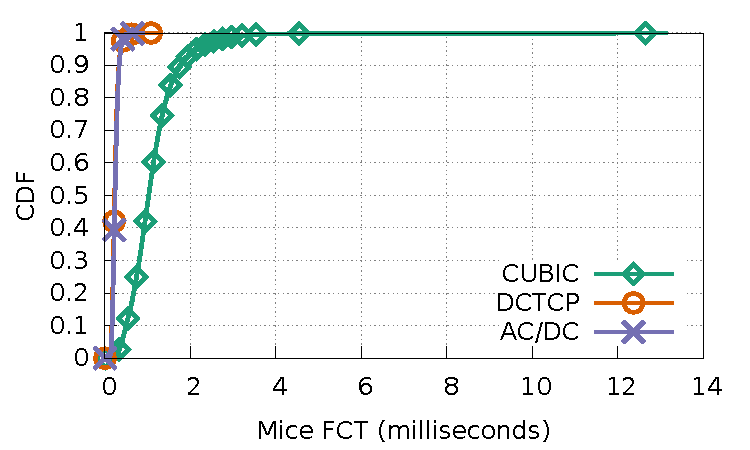
\includegraphics[width=\textwidth]{acdctcp/figures/macro_benchmarks/macro_4stride/stride4_mice16KB_fct.pdf}
                \caption{Mice flow completion times.}
                \label{macro_4stride_mice_fct}
        \end{subfigure}
        \begin{subfigure}[b]{0.45\textwidth}
                \centering
                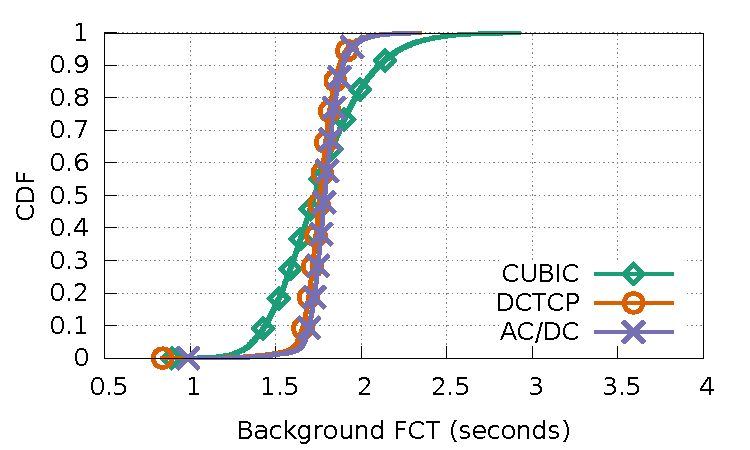
\includegraphics[width=\textwidth]{acdctcp/figures/macro_benchmarks/macro_4stride/stride4_big512MB_fct.pdf}
                \caption{Background flow completion times.}
                \label{macro_4stride_background_fct}
        \end{subfigure}
        \caption{CDF of mice and background FCTs in concurrent stride workload.}
        \label{macro_4stride_fct}
\end{figure*}

\begin{figure*}[!t]
        \centering
        \begin{subfigure}[b]{0.45\textwidth}
                \centering
                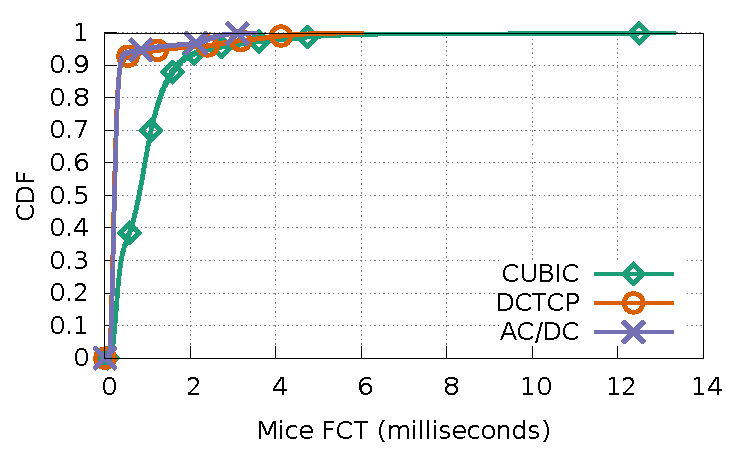
\includegraphics[width=\textwidth]{acdctcp/figures/macro_benchmarks/shuffle_17hosts/shuffle_mice16KB_fct.pdf}
                \caption{Mice flow completion times.}
                \label{macro_shuffle_mice_fct}
        \end{subfigure}
        \begin{subfigure}[b]{0.45\textwidth}
                \centering
                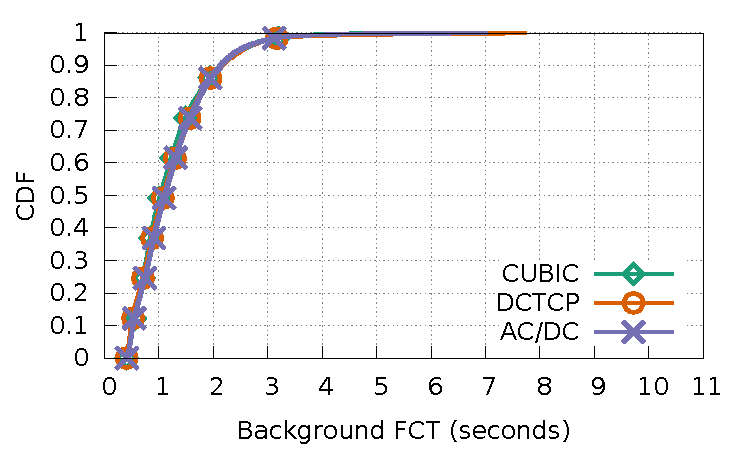
\includegraphics[width=\textwidth]{acdctcp/figures/macro_benchmarks/shuffle_17hosts/shuffle_big512MB_fct.pdf}
                \caption{Background flow completion times.}
                \label{macro_shuffle_background_fct}
        \end{subfigure}
        \caption{CDF of mice and background FCTs in shuffle workload.}
        \label{macro_shuffle_fct}
\end{figure*}

\begin{figure*}[!t]
        \centering
        \begin{subfigure}[b]{0.45\textwidth}
                \centering
                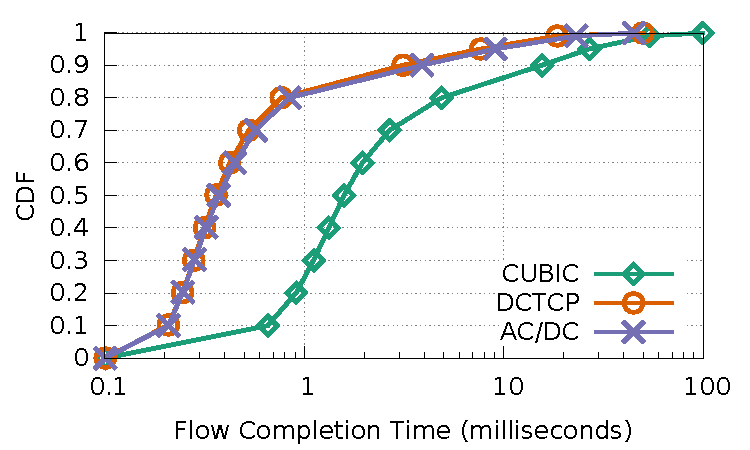
\includegraphics[width=\textwidth]{acdctcp/figures/macro_benchmarks/trace-driven/trace_driven_workload_dctcp_senders5_10points.pdf}
                \caption{Web-search workload.}
                \label{trace-driven-searching-fct}
        \end{subfigure}
        \begin{subfigure}[b]{0.45\textwidth}
                \centering
                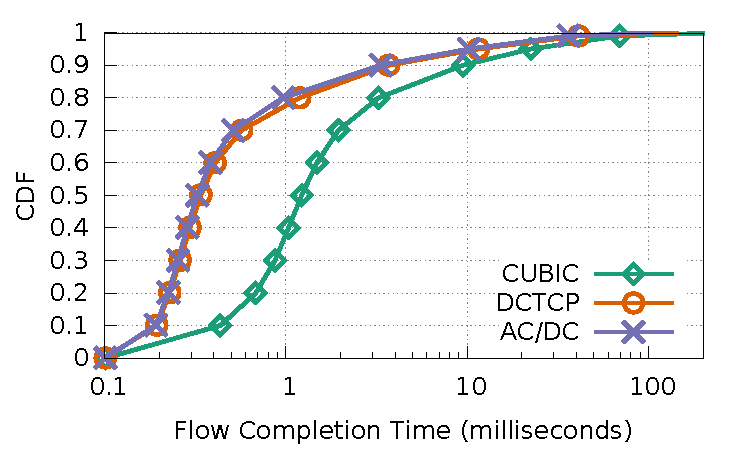
\includegraphics[width=\textwidth]{acdctcp/figures/macro_benchmarks/trace-driven/trace_driven_workload_conga_senders5_10points.pdf}
                \caption{Data-mining workload.}
                \label{trace-driven-data-mining-fct}
        \end{subfigure}
        \caption{CDF of mice (flows$<$10KB) FCT in web-search and data-mining workloads.}
        \label{macro-trace-driven-fct}
\end{figure*}

\tightparagraph{Concurrent stride workload}
In concurrent stride, 17 servers are attached to a single switch.
Each server $i$ sends a 512MB flow to servers [$i+1$, $i+4$] mod 17 in sequential fashion
to emulate background traffic.
Simultaneously, each server $i$ sends 16KB messages every 100 ms to 
server $(i+8)$ mod 17.
The FCT for small flows (16KB) and background flows (512MB) are shown 
in Figure~\ref{macro_4stride_fct}. For small flows, DCTCP and \acdc{} 
reduce the median FCT by 77\% and 76\% respectively. 
At the 99.9$^{th}$ percentile, DCTCP and \acdc{} reduce FCT by 91\% and 93\%, respectively.
For background flows, DCTCP and \acdc{} offer similar completion times.
CUBIC has longer background FCT because its fairness is not as 
good as DCTCP and \acdc{}.


\tightparagraph{Shuffle workload}
In shuffle, each server sends 512MB to every other server in random order. 
A sender sends at most 2 flows simultaneously and when
a transfer is finished, the next one is started until 
all transfers complete.
Every server $i$ also sends a 16 KB message to server $(i+8)$ mod 17 
every 100 ms. This workload is repeated for 30 runs.
The FCT for each type of flow is shown in Figure~\ref{macro_shuffle_fct}.
For small flows, DCTCP and \acdc{} reduce median FCT by
72\% and 71\% when compared to CUBIC. 
At the 99.9$^{th}$ percentile, DCTCP and \acdc{} 
reduce FCTs by 55\% and 73\% respectively.
For large flows, CUBIC, DCTCP and \acdc{} have almost identical performance.


\tightparagraph{Trace-driven workloads}
Finally, we run trace-driven workloads. 
An application on each server builds a long-lived TCP connection with every other server.
Message sizes are sampled from a trace and sent to a random destination in sequential fashion. Five
concurrent applications on each server are run to increase network load. Message
sizes are sampled from a web-search~\cite{alizadeh2011data}
and a data-mining workload~\cite{greenberg2009vl2,alizadeh2014conga}, whose flow size distribution has a heavier tail.
Figure~\ref{macro-trace-driven-fct} shows a CDF of FCTs for mice flows (smaller than 10KB) 
in the web-search and data-mining workloads.
In the web-search workload,
DCTCP and \acdc{} reduce median FCTs by 77\% and 76\%, respectively. 
At the 99.9$^{th}$ percentile, DCTCP and \acdc{} reduce FCTs by 50\% and 55\%, respectively.
In the data-mining workload, DCTCP and \acdc{} reduce median FCTs by 72\% and 73\%, respectively. 
At the 99.9$^{th}$ percentile, DCTCP and \acdc{} reduce FCTs by 36\% and 53\% respectively.  
%In both workloads, DCTCP and \acdc{} improve the fraction of mice flows that finish 
%in 1 millisecond significantly (from 20\%/30\% to 80\%).

\tightparagraph{Evaluation summary}
The results validate that congestion control can be accurately implemented in the vSwitch.
~\acdc{} tracks the performance of an unmodified host DCTCP stack
over a variety of workloads with little computational overhead.
Furthermore,~\acdc{} provides this functionality over 
various host TCP congestion control configurations. 


%\section{Discussion}
\label{discuss}

\tightparagraph{UDP traffic} How to handle. 
Mention VxLAN traffic too.
\keqiang{and IPsec}

\tightparagraph{No vSwitch} 
\keqiang{title should be hypervisor-bypass?}
Use middleboxes (for DB server).
Use NIC (for SR-IOV).
Hypervisor bypass (e.g., SR-IOV), where TCP traffic is sent to the NIC directly without 
going through hypervisor. First, as noted by~\cite{shieh2011sharing}, ``loss of the security and 
manageability features provided by the software virtual switch has limited 
the deployment of direct I/O NICs in public clouds''. Second, based on techniques like Intel 
DPDK~\cite{intel-dpdk} and ``smart NICs''~\cite{cavium-nic,netronome-nic}, we believe that low latency 
congestion control enforcement schemes like \acdc{} can also be 
employed for hypervisor bypass use cases.
We need to worry about legacy systems and non-VM systems. For instance, a database or storage device that may not have OVS installed on it.
We need to talk about either a middlebox or that this percentage of traffic is low? Or implement in NIC (especially one with OVS offload?).

\tightparagraph{North-South traffic.}
Transport enforcement should be only be done for east west traffic, so if the tenant tuned their stack's
congestion control algorithm for wide-area networks, their north sourth traffic is not affected and their 
congestion control scheme can still achieve good performance.

\keqiang{todos: some figures do not read well on printed paper}
\keqiang{todos: sometimes, when we refer a section, we say ``Section X'', sometimes, we use the 
dollar sign, we should unify them}

%
%Byzantine VM.
%
%Other names: ACDCTCP, LiquidSwitch, LiquidEdge
%
%In CPU overhead measurement, we need to 
%mention ovs add 1 widecard rule. That means we isolated the overhead of 
%OVS itself when it has many flows in its flow table (probably it does not matter
%at the end of the day, because we measured the CPU usage of the whole system).
%
%People may say window-based congestion control is burty. TIMELY operates 
%on TCP segments in order to reduce CPU overhead. Therefore, TIMELY is also
%busty. In TIMELY, they mentioned they can leverage a hybrid scheme, that is
%using software to control large segments and use hardware rate limiter to
%reduce burstyness.
%
%Create loss and check how DCTCP and our scheme treates packet losses (revisit it after we finish incast 
%and macrobenchmarks).
%
%One more microbenchmark on the Dumbbell topology: different servers have different transport, so the
%throughput fairness among different transports (e.g., start cubic, start New Reno, start dctcp).
%
%A point that is missing in DCTCP and NSDI paper is that they did not mention how the switch should be
%configured to handle non-TCP traffic. Note non-TCP traffic such as DNS (UDP 53) and ARP, ICMP etc
%are also important. We found that if we did not specify how the switch handle the non-TCP traffic,
%then this kind of non-TCP traffic can be easily dropped by the switch. We found ARP traffic is dropped
%by the switch such that DCTCP flows stall. Hence, we think it is better to put non-TCP traffic
%into a different queue when we apply WRED/ECN on the switches.
%
%This work offers low latency for ``hetergeneous networks" where different entities can 
%run different kinds of
%transport congestion control schemes. A few examples of such hetergeneous networks: public 
%datacenters where tenants can set up their own VMs (e.g., AWS), or tenants can rent their bare metal
%machines (e.g., SoftLayer), or certain groups (even within a single organization) 
%have to use traditional transports due to compatibility of legacy applications (NSDI's Judd said this), or
%incremental deployment is undergoing. 
%To ensure a pure low latency datacenter network, a universal transport enforcement scheme is required. 
%Two challenges to implement such a transport enforcement scheme are scalability and low overhead. 
%The transport enformancement scheme proposed here meet the two metrics (as shown in our experiments) while
%providing nice network performance (throughput, latency and packet drop rate). This scheme is 
%compatible with any kind of TCP stack. Finally, the scheme we propose solves the co-existence issue of 
%ECT (ECN Capable Transport) and non-ECT, which is a critical deployment hurdle for DCTCP-like transports.
%
%Macrobenchmark plan: 18 hosts, 6 switches, ECMP configured. The network oversubscription ratio is 2:1.
%Run all-to-all traffic for a long time (e.g., 1 hours). Show total throughput and TCP RTT and packet drop 
%rate.
%
%QoS can be implemented too?
%
%
%
%When we try to launch an instance in EC2: ``An AMI is a template that contains the software 
%configuration (operating system, application server, and applications) required to launch your instance. 
%You can select an AMI provided by AWS, our user community, or the AWS Marketplace; 
%or you can select one of your own AMIs''. Default is CUBIC for most Linux images, Window Servers can
%have NewReno, Compound TCP (CTCP)~\cite{tan2006compound} and DCTCP. 
%Users can tweak congestion control algorithms to optimize network performance for their target scenarios. 
%
%Section talking about how to implement other CC schemes: TIMELY, PERC, Vegas, etc.
%
%EJR: VXLAN, UDP, TCP stack statistics for Cloud?
%
%ECT and non-ECT: througput unfairness, long RTT, connection establishment..
%
%
%EyeQ, Seawall, NetShare, Silo, SecondNet, Oktopus etc. Our work did not provide bandwidth allocation property. 
%This work focused on reducing in-network queuing latency caused by VM TCP stacks. 
%We show how this goal can be done using a simple and elegant solution.
%Yes, if an VM opens more connections than another, that VM gains more bandwidth. 
%But, there are proposals which try to provide proper bandwidth allocation when multiple end-points compete 
%at the sender side or receiver side. Those works and this work are complementary. 
%To the best of our knowledge, today's cloud providers have not provide strong bandwidth guarantees 
%(for example, AWS only roughly classify VMs instances' network performance into 
%``low to moderate", ``moderate", ``high" and ``10 Gigabit"categories).
%
%talk about containers?


{\bf Load Balancing in Datacenters} 
%Load balancing in datacenter networks has been the focus of several studies.
MPTCP~\cite{mptcp,dc-mptcp} is a transport protocol that uses subflows to 
transmit over multiple paths.
CONGA~\cite{conga} and Juniper VCF~\cite{juniper-vcf} both employ congestion-aware flowlet switching~\cite{flowlet} on
specialized switch chipsets to load balance the network.
RPS~\cite{packetspray} and DRB~\cite{drb} evaluate per-packet load balancing on symmetric 1 Gbps networks
at the switch and end-host, respectively.
The CPU load and feasibility of end-host-based per-packet load balancing for 10+ Gbps networks remains open.
%Per-packet load balancing can incur significant end-host overhead for DRB
%if not resorting to jumbo frames.
%Packet reordering problem is not well considered in both RPS and DRB.
%RPS and DRB may perform worse than ECMP in case of topology asymmetry.
Hedera~\cite{hedera}, MicroTE~\cite{microte} and Planck~\cite{planck} use centralized traffic engineering to
reroute traffic based on network conditions.
FlowBender~\cite{flowbender} reroutes flows when congestion is detected by end-hosts and 
Fastpass~\cite{fastpass} employs a centralized arbiter to schedule path selection for each packet.
As compared to these schemes, Presto is the only one that proactively load-balances at line rate for fast networks
in a near uniform fashion without requiring additional infrastructure or changes
to network hardware or transport layers. Furthermore, to the best of our knowledge, Presto is
the first work to explore the interactions of fine-grained load balancing with built-in
segment offload capabilities used in fast networks.
%\textcolor{blue}{~\cite{eden} also advocates to implement network functions such as load balancing 
%at datacenter end hosts.}

{\bf Reducing Tail Latency}
%Detail~\cite{detail} summarizes the causes of long tails of flow completion time---
%1)packet loss and retransmissions,
%2)absence of flow prioritization and 3)uneven load balancing.
%Reducing tail latencies of small mice flows has also been actively studied.
DeTail~\cite{detail} is a cross-layer network stack designed to reduce the tail of flow completion times.
%link layer uses port buffer occupancy to construct lossless fabric,
%network layer performs per-packet adaptive load balancing based on port buffer occupancy,
%transport layer relies upon congestion notifications
%derived from port buffer occupancies,
%finally Detail lets application layer specify flow priorities to
%avoid head-of-line blocking of elephant flows for mice time-sensitive flows.
%Detail modified many layers (including the switch) and is hard to deploy using
%current hardware and network stack.
DCTCP~\cite{dctcp} is a transport protocol that uses the portion of marked packets 
by ECN to adaptively adjust sender's TCP's congestion window to reduce switch buffer occupancy.
%Thus, DCTCP can reduce switch buffer occupancy and reduce flow completion time.
HULL~\cite{hull} uses Phantom Queues and congestion notifications to cap link utilization and prevent congestion.
%HULL uses packet pacing to combat with traffic burstiness in order to leave "bandwidth headroom".
In contrast, Presto is a load balancing system that naturally improves 
the tail latencies of mice flows by uniformly spreading traffic in 
fine-grained units.
%We share the overall goal of reducing mice tail latencies, but instead explore how
%fine-grained load balancing can provide a solution.
QJUMP~\cite{qjump} utilizes priority levels to 
allow latency-sensitive flows to "jump-the-queue" over low priority flows.
PIAS~\cite{bai2015information} uses priority queues to mimic the Shortest Job First principle to reduce FCTs.
%solve the network interference problem caused by elephant and mice flows 
%for datacenter networks. High priority packets are rate-limited 
%at the end-host and can "jump-the-queue" over packets with 
%lower priorities. PIAS~\cite{pias} mimics the Shortest Job First (SJF) 
%principle to reduce flow completion times. It gradually decreases 
%the priority level assigned to a flow based on its flow size.
%Presto is complementary and could be applied on each priority level.
%DIBS~\cite{dibs} detours packets of a congested switch port to a randomly 
%picking neighboring switch to reduce packet drops.
Last, a blog post by Casado and Pettit~\cite{vmware} summarized
four potential ways to deal with elephants and mice, with one advocating
to turn elephants into mice at the edge. 
We share the same motivation and high-level
idea and design
a complete system that addresses many practical challenges of using
such an approach.


{\bf Handling Packet Reordering}
%Many schemes have tried to mitigate the impact of reordering.
TCP performs poorly in the face of reordering, and thus several studies
design a more robust alternative~\cite{rr-tcp,blanton2002making,tcp-pr}.
Presto takes the position that reordering should be handled below TCP in the existing 
receive offload logic.
In the lower portion of the networking stack, SRPIC~\cite{wu2009sorting} sorts reordered packets 
in the driver after each interrupt coalescing event. While this approach can help
mitigate the impact of reordering, it does not sort packets across interrupts, have a 
direct impact on segment sizes, or distinguish between loss and reordering. 
%SRPIC is 
%complementary to our approach because their actions are taken in the driver, before packets
%are pushed to GRO.
%RR-TCP~\cite{rr-tcp} proposed to extend TCP sender to detect and recover from false fast retransmits using DSACK information. 
%As we show, fixing TCP itself cannot solve all the problems incurred by packet reordering.
%\eric{i have some LRO references in the patent slides that we need to make sure are cited somewhere} 
%Instead, Presto's chunking scheme leverages the fact that all the packets going through the same path are in order and has two nice properties:
%1)Presto uses chunkid to make the task of distinguishing packet loss from temporary packet reordering much simpler. 
%2)Presto only needs to make sure the chunks are in order instead of packets, thus reducing per-packet processing overhead.

{\bf Congestion control for DCNs}
%\crs{Rather than proposing a new congestion control algorithm, our work investigates if congestion control can be moved to the vSwitch.
%Thus, many of the following schemes are complimentary.}
DCTCP~\cite{dctcp} is a seminal TCP variant for datacenter networks.
Judd~\cite{judd2015nsdi} proposed simple yet practical fixes to enable DCTCP in production networks.
TCP-Bolt~\cite{stephens2014practical} is a variant of DCTCP for PFC-enabled lossless Ethernet.
%DCQCN~\cite{zhu2015congestion} is a rate-based congestion control scheme implemented in NICs
%for QCN-based~\cite{qcn} RDMA deployments.
DCQCN~\cite{zhu2015congestion} is a rate-based congestion control scheme (built on DCTCP and QCN) to
support RDMA deployments in PFC-enabled lossless networks.
TIMELY~\cite{mittal2015timely} and DX~\cite{lee2015accurate}
use accurate network latency as the signal to perform congestion control.
TCP ex Machina~\cite{winstein2013tcp} uses computer-generated congestion control rules.
PERC~\cite{jose2015high} proposes proactive congestion control to improve convergence.
ICTCP's~\cite{wu2010ictcp} receiver monitors incoming TCP flows and
modifies~\rwnd{} to mitigate the impact of incast, but this cannot
provide generalized congestion control like~\acdc{}.
Finally, efforts~\cite{dell-toe,chelsio-toe} to
implement TCP Offload Engine (TOE) in specialized NICs are not widely deployed for reasons noted in~\cite{mogul2003tcp,linux-toe}.
vCC~\cite{vcc} is a concurrently designed system that shares~\acdc{}'s goals and some of its design details.
The paper is complementary in that some items not addressed in~\acdc{} are presented, such as a more detailed
analysis of the ECN-coexistence problem, an exploration of the design space, and a theoretical proof of
virtualized congestion control's correctness.~\acdc{} provides an in-depth design and thorough evaluation of
a DCTCP-based virtualized congestion control algorithm on a 10 Gbps testbed.


{\bf Bandwidth allocation} Many bandwidth allocation schemes have been proposed.
Gatekeeper~\cite{rodrigues2011gatekeeper} and EyeQ~\cite{jeyakumar2013eyeq} abstract the network as a single
switch and provide bandwidth guarantees by managing each server's access link.
Oktopus~\cite{Ballani2011oktopus} provides fixed performance guarantees within virtual clusters.
SecondNet~\cite{Guo2010Secondnet} enables virtual datacenters with static bandwidth guarantees.
Proteus~\cite{Xie2012Proteus} allocates bandwidth for applications with dynamic demands.
Seawall~\cite{shieh2011sharing} provides bandwidth proportional to a defined weight by
forcing traffic through congestion-based edge-to-edge tunnels.
NetShare~\cite{Lam2012NetShare} utilizes hierarchical weighted max-min fair sharing to tune relative bandwidth allocation for services.
FairCloud~\cite{Popa2012Faircloud} identifies trade-offs in minimum
guarantees, proportionality and high utilization, and designs schemes over this space.
Silo~\cite{jang2015silo} provides guaranteed bandwidth, delay and burst allowances through a novel VM placement and admission
algorithm, coupled with a fine-grained packet pacer. 
~\acdc{} is largely complimentary to these schemes because it is a transport-level solution.

{\bf Rate limiters}
SENIC~\cite{niranjan2013fastrak}
identifies the limitations of NIC hardware rate limiters (\ie{}, not scalable) and
software rate limiters (\ie{}, high CPU overhead) and uses the CPU to enqueue packets
in host memory and the NIC. Silo's pacer injects void packets into
an original packet sequence to achieve pacing. FasTrack~\cite{niranjan2013fastrak} offloads
functionality from the server into the switch for certain flows.
%~\acdc{} prevents
%TCP flows from sending in the first place and can be used in conjunction with these
%schemes.


\section{Summary}
\label{sec:conclusion}
In this chapter, we present Presto: a near uniform sub-flow distributed load balancing scheme
that can near optimally load balance the network at fast networking speeds.
Our scheme makes a few changes to the hypervisor soft-edge (vSwitch and GRO)
and does not require any modifications to the transport layer or network hardware, making
the bar for deployment lower. 
%Working at fast networking speeds poses many challenges,
Presto is explicitly designed to load balance the network at fine granularities
and deal with reordering without imposing much overhead on hosts. Presto is flexible and can also
deal with failures and asymmetry. Finally, we show the performance of Presto can closely track
that of an optimal non-blocking switch, meaning elephant throughputs remain high while the tail
latencies of mice flow completion times do not grow due to congestion.


\section*{Acknowledgement}

\crs{We would like to thank our shepherd Vishal Misra, Jeff Rasley, Brent Stephens and
the anonymous reviewers for their valuable feedback. This
work is supported in part by National
Science Foundation (grants CNS-1302041, CNS-1330308
and CNS-1345249), IBM Corporation and the Wisconsin Institute on Software-Defined Datacenters of Madison.}

\balance
{%\scriptsize
\small
\setlength{\bibsep}{0.5pt}
\raggedright
\bibliographystyle{abbrv}
\bibliography{refer}
}

\end{document}
